% !TEX TS-program = pdflatexmk

%\documentclass[12pt,oneside,reqno]{amsart}
\documentclass[12pt]{article}
\usepackage[reqno]{amsmath}
\usepackage{geometry} % see geometry.pdf on how to lay out the page. There's lots.
\geometry{a4paper} % or letter or a5paper or ... etc
\usepackage[titletoc,toc,title]{appendix}
\usepackage{lipsum}
\usepackage{filecontents}
\usepackage[dvipsnames]{xcolor}
\usepackage[utf8]{inputenc}
\usepackage[framed,numbered,autolinebreaks,useliterate]{mcode}
% \geometry{landscape} % rotated page geometry
%% LaTeX Preamble - Common packages
%\usepackage[margin=1in]{geometry}
\usepackage{graphicx}
%% LaTeX - Article customise
%%% PACKAGES
\usepackage{booktabs} % for much better looking tables
\usepackage{array} % for better arrays (eg matrices) in maths
\usepackage{paralist} % very flexible & customisable lists (eg. enumerate/itemize, etc.)
\usepackage{verbatim} % adds environment for commenting out blocks of text & for better verbatim
% make it possible to include more than one captioned figure/table in a single float
% These packages are all incorporated in the memoir class to one degree or another...
%% LaTeX Preamble - Common packages


 % Put the bibliography in the ToC
 % Alter the style of the Table of Contents
% Swap the definition of \abs* and \norm*, so that \abs
% and \norm resizes the size of the brackets, and the 
% starred version does not.

 % Any characters can be typed directly from the keyboard, eg ���
\usepackage{textcomp} % provide lots of new symbols
%\usepackage{epstopdf} % to include .eps graphics files with pdfLaTeX
\usepackage{flafter}  % Don't place floats before their definition
%\usepackage{topcapt}   % Define \topcation for placing captions above tables (not in gwTeX)
\usepackage{natbib} % use author/date bibliographic citations
\usepackage{subfig}
\usepackage{amsmath,amssymb}  % Better maths support & more symbols
\usepackage{bm}  % Define \bm{} to use bold math fonts

 % PDF hyperlinks, with coloured links
\usepackage[pdftex,bookmarks,colorlinks,breaklinks]{hyperref} 

\newcommand\myshade{85}
\colorlet{mylinkcolor}{NavyBlue}
\colorlet{mycitecolor}{YellowOrange}
\colorlet{myurlcolor}{violet}

\hypersetup{
  linkcolor  = mylinkcolor!\myshade!black,
  citecolor  = mycitecolor!\myshade!black,
  urlcolor   = myurlcolor!\myshade!black,
  colorlinks = true,
}
%%% PAGE DIMENSIONS
 % for example, change the margins to 2 inches all round
\usepackage{cleveref}
%\geometry{landscape} % set up the page for landscape
% read geometry.pdf for detailed page layout information

%%% HEADERS & FOOTERS
\usepackage{fancyhdr} % This should be set AFTER setting up the page geometry
\pagestyle{fancy} % options:empty , plain , fancy
\renewcommand{\headrulewidth}{0pt} % customise the layout...
\lhead{}\chead{}\rhead{}
\lfoot{}\cfoot{\thepage}\rfoot{}
\usepackage{tocloft}
\setcounter{secnumdepth}{-2}
  %% END Article customise
\renewcommand{\thesection}{}
\usepackage{multicol}

\newcommand{\abs}[1]{\left\lvert#1\right\rvert}
\newcommand{\norm}[1]{\left\lVert#1\right\rVert}
\title{Brain Machine Interaction \\ Feedback Modality for motor imagery practice}

\author{
Jaquier. M, Jeanningros. L
\\
EPFL \\
}

\nipsfinalcopy 

\begin{document}
\maketitle
\tableofcontents
\newpage

\begin{multicols}{2}
\section{Introduction}
Over the last 15 years there has been a great deal of speculation into the potential for electroencephalographic (EEG) measurements providing an alternate channel for information transfer from the brain to external devices \cite{clinical}. Brain Machine Interfaces (BCI) are of growing interest as a method to control tools, robotics, or damaged limbs in a novel fashion. The majority of research focuses mainly on subjects suffering from traumatic injury \cite{murphy}; to that end functional electrical stimulation (FES) has proven effective in assisting patients with injuries that prevent normative movement of limbs \cite{Pfurtscheller200333}. 

Most BCI systems use EEG signals measured from scalp electrodes due in large part to the non-invasive nature of the procedure. Motor imagery (MI) has been widely studied and has proven a strongly discriminable signal from EEG recordings \cite{MI}, however controlling device through a BCI appears laborious to learn \cite{Curran2003326}; despite the potential difficulty for subjects attempting to control the BCI through MI it remains one of the most widely utilised and studied methods. Feedbacks is widely regarded as a principal component of the learning processes \cite{Mitz:1991aa}. Many of the studies have employed visual feedback to assist the subject during the training phases, while somewhat effective the learning is diluted by the additional mental processing necessary to integrate visual feedback. The present study considers sensorimotor feedback, in the form of functional electrical stimulation, as a potential source of feedback. This work aims to understand the impact of FES on modulation of brain oscillations, to extract meaningful features and design a classifier discriminating motor imagery from resting tasks and to evaluate the impact of the feedback modality on the BCI performance.


\section{Methods}
\subsection{Protocol}

Two healthy subjects performed three sessions the first two sessions were in either the visual (no FES) modality or the FES modality, each session was broken down into four sets of thirty trials each, the third and final session was composed of two sets with FES and visual modalities, and one set of FES with no MI to be used as a control. Subjects were seated approximately one meter in front of a screen positioned at eye level during EEG recordings.  A single trial corresponds to a visual cue indicating the requested task. The two different task - MI and rest - were randomly ordered so that the subject performs 15 MI tasks and 15 resting tasks.

During FES trials three electrodes are to the subjects arm, two stimulating electrodes on the forearm and a ground electrode is placed on the biceps in order to attenuate the noise introduced by FES recorded at the level of the EEG apparatus. During resting tasks no stimulation is applied, during motor imagery tasks, a small electrical stimuli is present throughout the trial, a stimulus with enough amplitude to cause muscular contraction is applied at the end of the trial resulting in artificial hand grasping.

The EEG features are composed of 64 channels, later filtered to 16 channels of interest, channels are recorded at 512 Hz at measured scalp positions. The \textit{Cz}-electrode is centred on the scalp midway between the nasion and inion, the ear electrodes are used as references and the \textit{AFz} electrode utilised as the ground electrode. Before each session, the ratio signal over noise is verified. A gel enables to ensure a good connectivity between every electrodes and the scalp. Recorded data is saved alongside the appropriate label as either rest, or MI in order to facilitate classifier training, and headers in order to distinguish between trials.

\subsection{Preprocessing}

The original signal was referenced utilising the ear electrodes. Epoching the data is carried out by extracting data points referenced by the header, each segment is referred to as a single trial. Trials with \textit{NaN} are purged in order to avoid contaminating the data during downstream processing.  Each trial has a corresponding label designating which task was performed by the subject for that trial. We zero our baseline by subtracting the mean of the signal.. The function \textit{detrend} from \textbf{Matlab} is appropriate to this task. Depending on the selected option, it can remove the mean value of a vector, but also a linear trend. We choose that second option for each channel of each trial (fig.\ref{Off_detrend}).

%\begin{figure}
%\begin{center}
%\includegraphics[scale=0.35]{Off1.eps}
%\caption{Signal of the 16 channels from a single trial}
%\label{Off1}
%\end{center}
%\end{figure}

\begin{figure*}
\begin{center}
\subfloat[Before removing linear trend]{\includegraphics[scale=0.33]{Off_detrend1.eps}}
\quad
\subfloat[After removing linear trend]{\includegraphics[scale=0.33]{Off_detrend2.eps}}
\end{center}
\caption{Effect of the \textit{detrend} function}
\label{Off_detrend}
\end{figure*}

Spatial filtering it employed to accurately depict the diffuse nature of the EEG signal. The skull being bone has a significantly greater attenuation coefficient compared to the softer brain matter, thus much of the EEG signal is dispersed across the surface of the skull by some distance. We attempt to correct for the electrical diffusion across the skulls surface by filtering the data utilising one of two spatial filters. 

Common Average Reference (CAR). The average of all channels at a time is removed from each channel. CAR is employed to remove similarities over all recording electrodes. \begin{equation}
u_i^{CAR} = u_i - \frac{1}{n} \sum_{j=1}^n u_j
\label{eq:1}
\end{equation}
where $u_i$ is the potential of channel $i$

Laplacian filtering. The laplacian operator measures the spatial second derivative, laplacian filtering highlights regions of rapid intensity change and is therefore commonly employed for edge detection. Filtering with the laplacian operator reduces similarities across a region of the space and underlines frontiers. The laplacian can be more or less large depending on the structure and the number of electrodes composing the map. For the sake of our work we have found the small laplacian transform, where we utilise immediate neighbours, to be most effective. 
\begin{equation}
u_i^{LAP} = u_i- \sum_{j \in S_i} h_{ij} u_j
\label{eq:2}
\end{equation}
where $S_i$ is the defined neighbourhood of channel $i$ and $h_{ij}$ the distance between electrodes $i$ and $j$ normed over all the sum of distances. The term small laplacian is used when the neighbourhood is the 4 nearest neighbourhood and large laplacian when it takes the 4 second-neighbourhood.

\subsection{Feature extraction}

The nature of the EEG signal lends it self to calculations in the frequency domain. Given that EEG recordings represent large population of neurons that can lead to synchronisation or desynchronisation measurable by EEG recordings. This behaviour is amenable to discrimination via analysis of the power spectral density (PSD) since (de)synchronisation appears as a change of density in a specific frequency band. The method consists of a Fourier transform on a time window (epoch) of consistent length, with a given overlap for signal smoothing. Overlapping the PSD windows smooths the resulting data, care must be taken to not abuse the overlap size as information is lost during the smoothing process, for our data a 50 percent overlap is utilised in accordance with common literature practices \cite{1741-2552-4-2-R01}. The \textbf{Matlab} function \textit{pwelch} has been used for our analysis. 
 \begin{lstlisting}
 [pdata, ~] = pwelch(data, window_size,window_ol, freq_space, sample_freq)
 \end{lstlisting}
 
 
\subsection{Feature selection}

The feature space provided by PSD is proportional to the frequency space provided to the \textit{pwelch} function of Matlab. We prune this feature space down to a select few relevant features by the use of three statistical methods. 

Linear correlation coefficient. A widely utilised statistical method in order to ascertain correlation between two data sets. We utilise the Pearson product-moment:
\begin{equation}
\rho(X,Y) = \frac{{\bf
Cov}(X,Y)}{\sqrt{{\bf Var}(X){\bf Var}(Y)}}
\label{eq:e3}
\end{equation}

Fisher score. Fisher scoring is widely used throughout literature for BCI feature selection, it is robust, rapid, and provides a less noisy picture of information content relative to the linear correlation coefficient. There exists a multitude of formulas to calculate the Fisher score, we chose a formulation which was utilised specifically for the problem of feature selection in machine learning \cite{he2005laplacian}. 

\begin{equation}
F_r = \frac{\sum_{i=1}^c n_i(\mu_i - \mu)^2}{\sum_{i=1}^c n_i \sigma_i^2}
\label{eq:e4}
\end{equation}

\subsection{Classifier}

Three classifiers were compared in order to assess the best performance manageable. We chose classifiers that were frequently utilised throughout literature in order to maximise our ability to compare the results of our FES study to similar studies which employ different forms of feedback. 

Linear Discriminant Analysis (LDA). LDA is very commonly used as a classifier due to the simplicity of interpreting the results and the low computational costs of training. LDA makes several assumptions which are of key importance. First it will assume the data is generated as a gaussian distribution, second it assumes the covariance matrices of the data sets are the same. 

Quadratic Discriminant Analysis (QDA). QDA is implemented with the exact same mathematical formulation with the exception that the covariance matrix between labels is not assumed to be the same. This allows QDA to take decision boundaries which are non-linear. This property makes QDA more flexible than LDA but at the cost of additional computational expense. 

\begin{equation}
D(x) = wx + b
\label{lda1}
\end{equation}
Where w is the normal vector and b is a threshold, they are determined by maximising the between, and with class variance. 
\begin{equation}
S_b = \sum_{i=1}^K(u_i - u_c)(u_i - u_c)^T
\label{lda2}
\end{equation}
Where $u_c$ is the mean of the data set, K is the number of labels, and $u_i$ is the expected value of the class $i$. 
\begin{equation}
S_w = \sum_{i=1}^K\sum_{l=1}^N_i(x_l - u_i)(x_l - u_i)^T
\label{lda3}
\end{equation}
Where $N_i$ is the number of samples with label $i$ \cite{fisher1936use}. The above equations are utilised in both LDA and QDA with the explicit difference being that LDA assumes a single covariance matrix. 


Support Vector Machine (SVM). SVM classifies exact two data sets by finding a hyperplane which maximises the distance between the two sets of data. The support vectors are those data points which are closest to the hyperplane formed by the SVM. In order to address cross-study we utilise the more common SVM algorithm,  Sequential Minimal Optimisation (SMO) and a linear kernel. Successful training of an SVM requires careful selection of the correct kernel.
\begin{equation}
y = \operatorname{sgn}(\sum_{i=1}^N y_i a_i k(x_i \cdot x) +b)
\label{svm1}
\end{equation}
Where $\big\{x_i,y_j\big\}_{i=1}^N$ is our data, and $a_i$ are Lagrangian multiplies from solving the optimisation problem, $k(x_i,x_j)$ is the kernel function, and $b$ is the bias \cite{xu2011robot}. Note here that by utilising SMO our SVM is utilising a linear, not quadratic, optimisation method. 

\section{Results}
\subsection{Subject 1}
After calculation of the PSD we assess the quality of the data by evaluating the mean of each channel and plotting it. From (fig.\ref{meanPSD}) it becomes apparent that the FES feedback modality introduces a great deal of noise around 30Hz that must be filtered out in order to extract any useful features from the data.   

\begin{figure*}
\begin{center}
\subfloat[Ch 12 PSD S1]{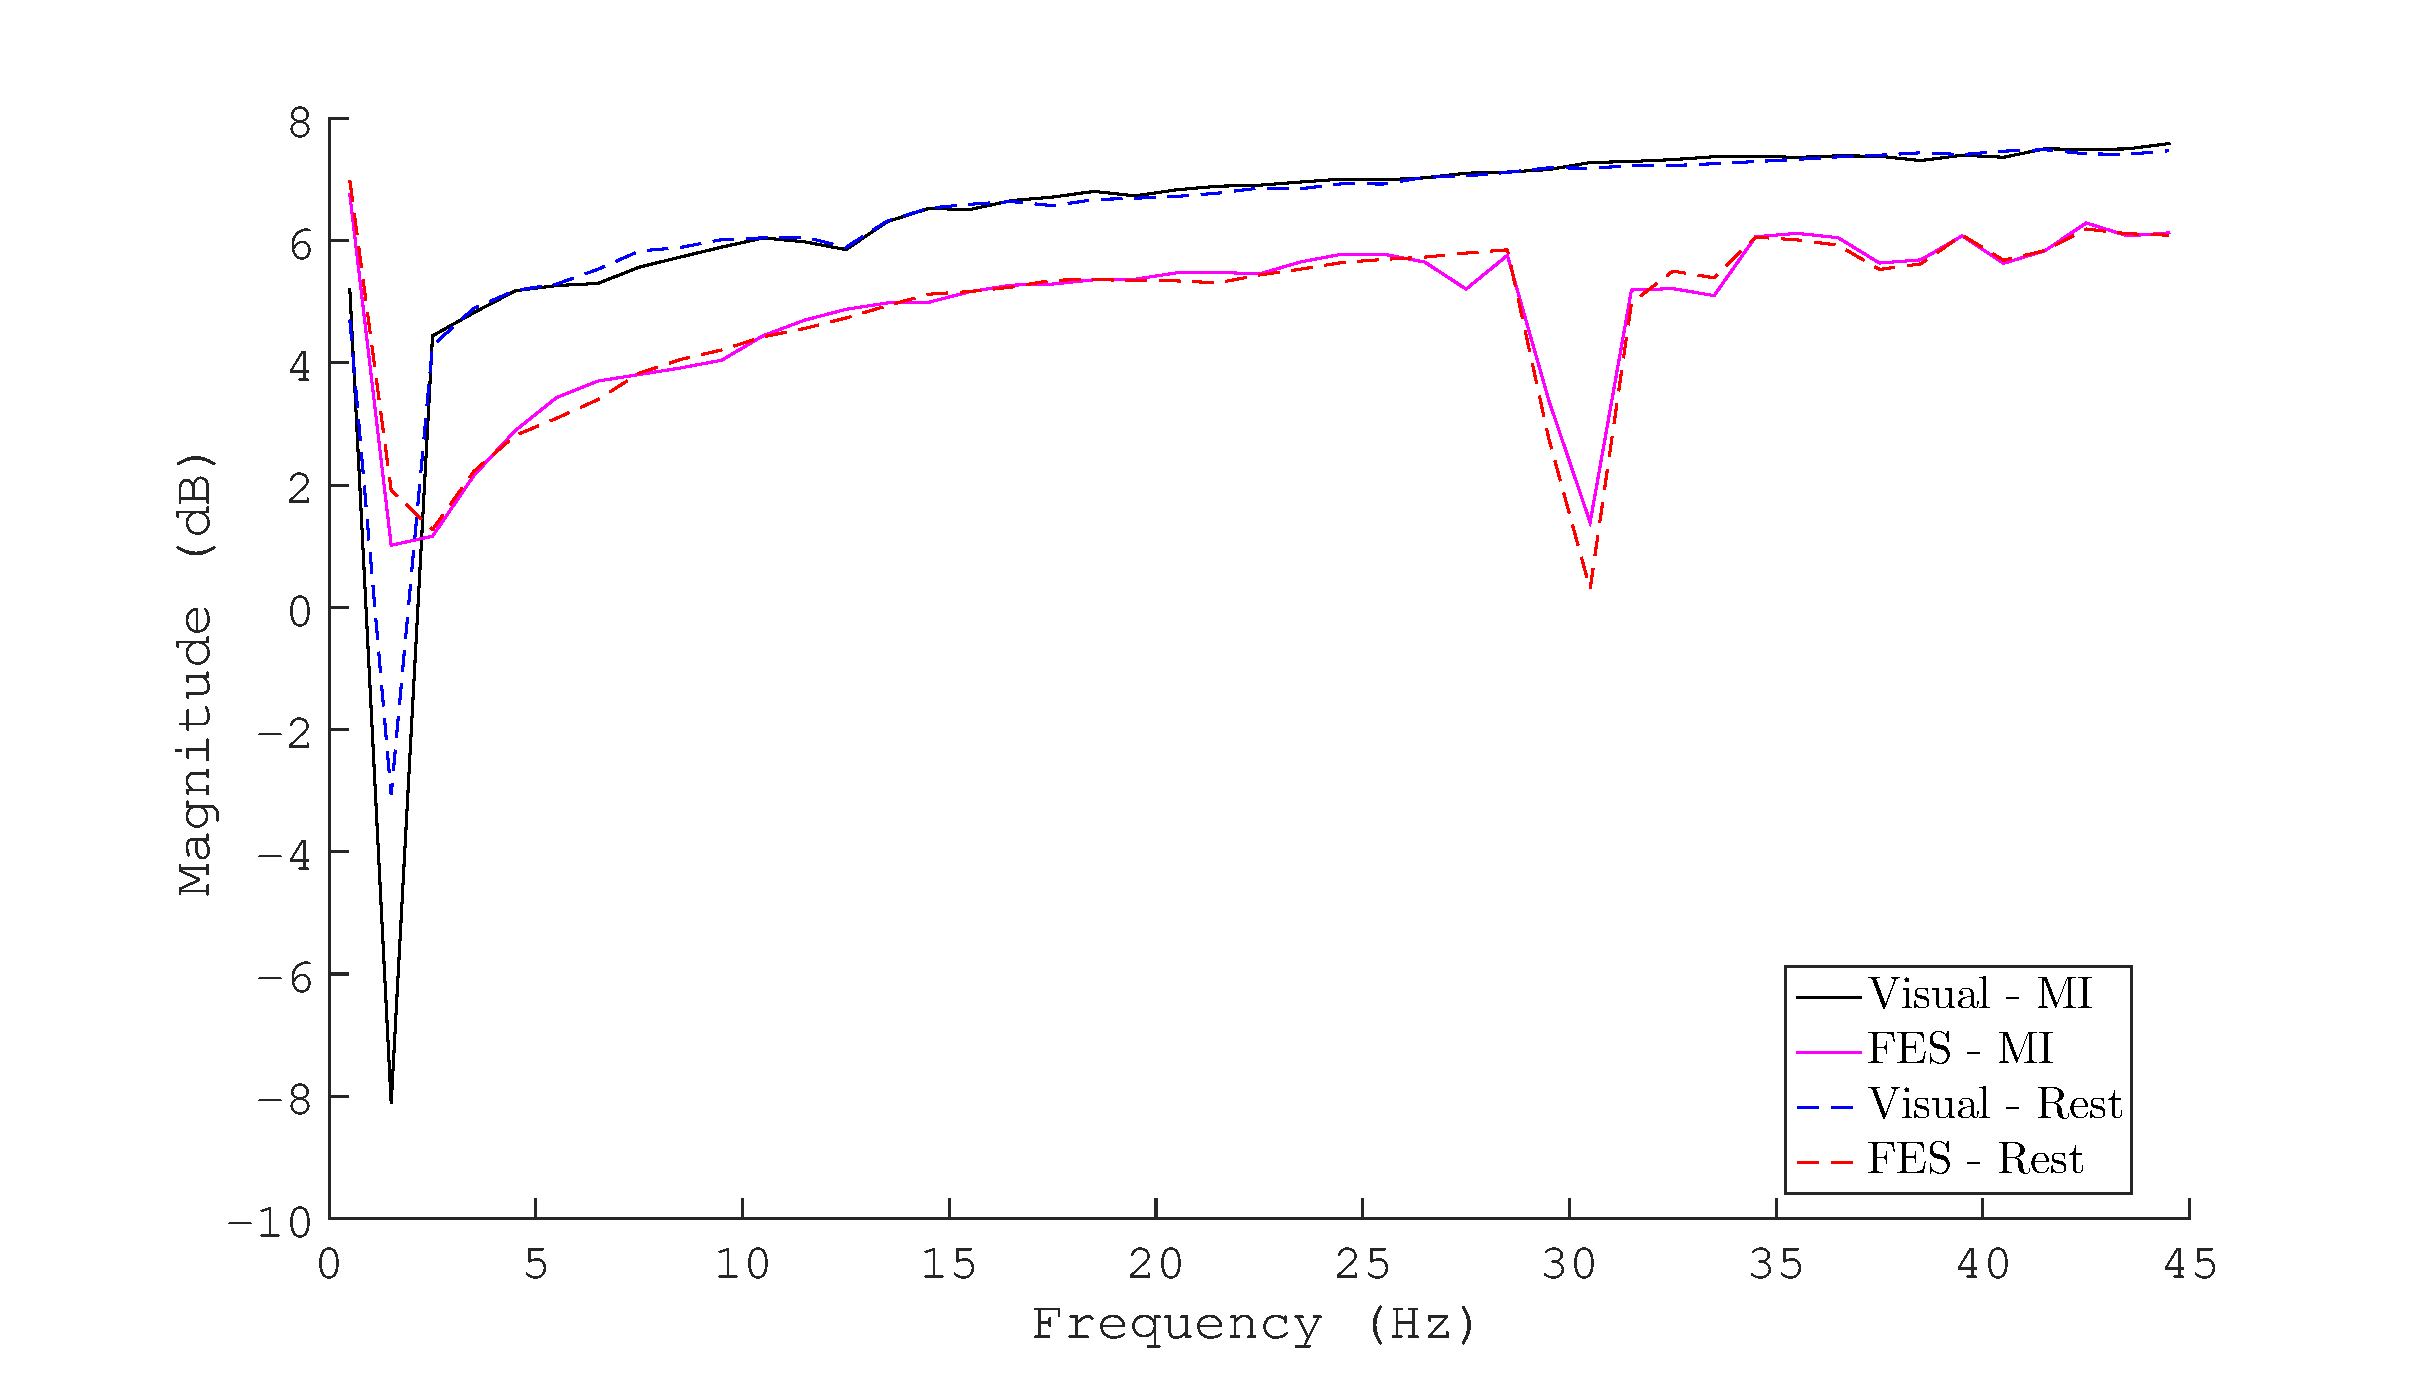
\includegraphics[width=.9\textwidth]{fig/ele12.eps}}
\qquad
\subfloat[Ch 12 PSD S2]{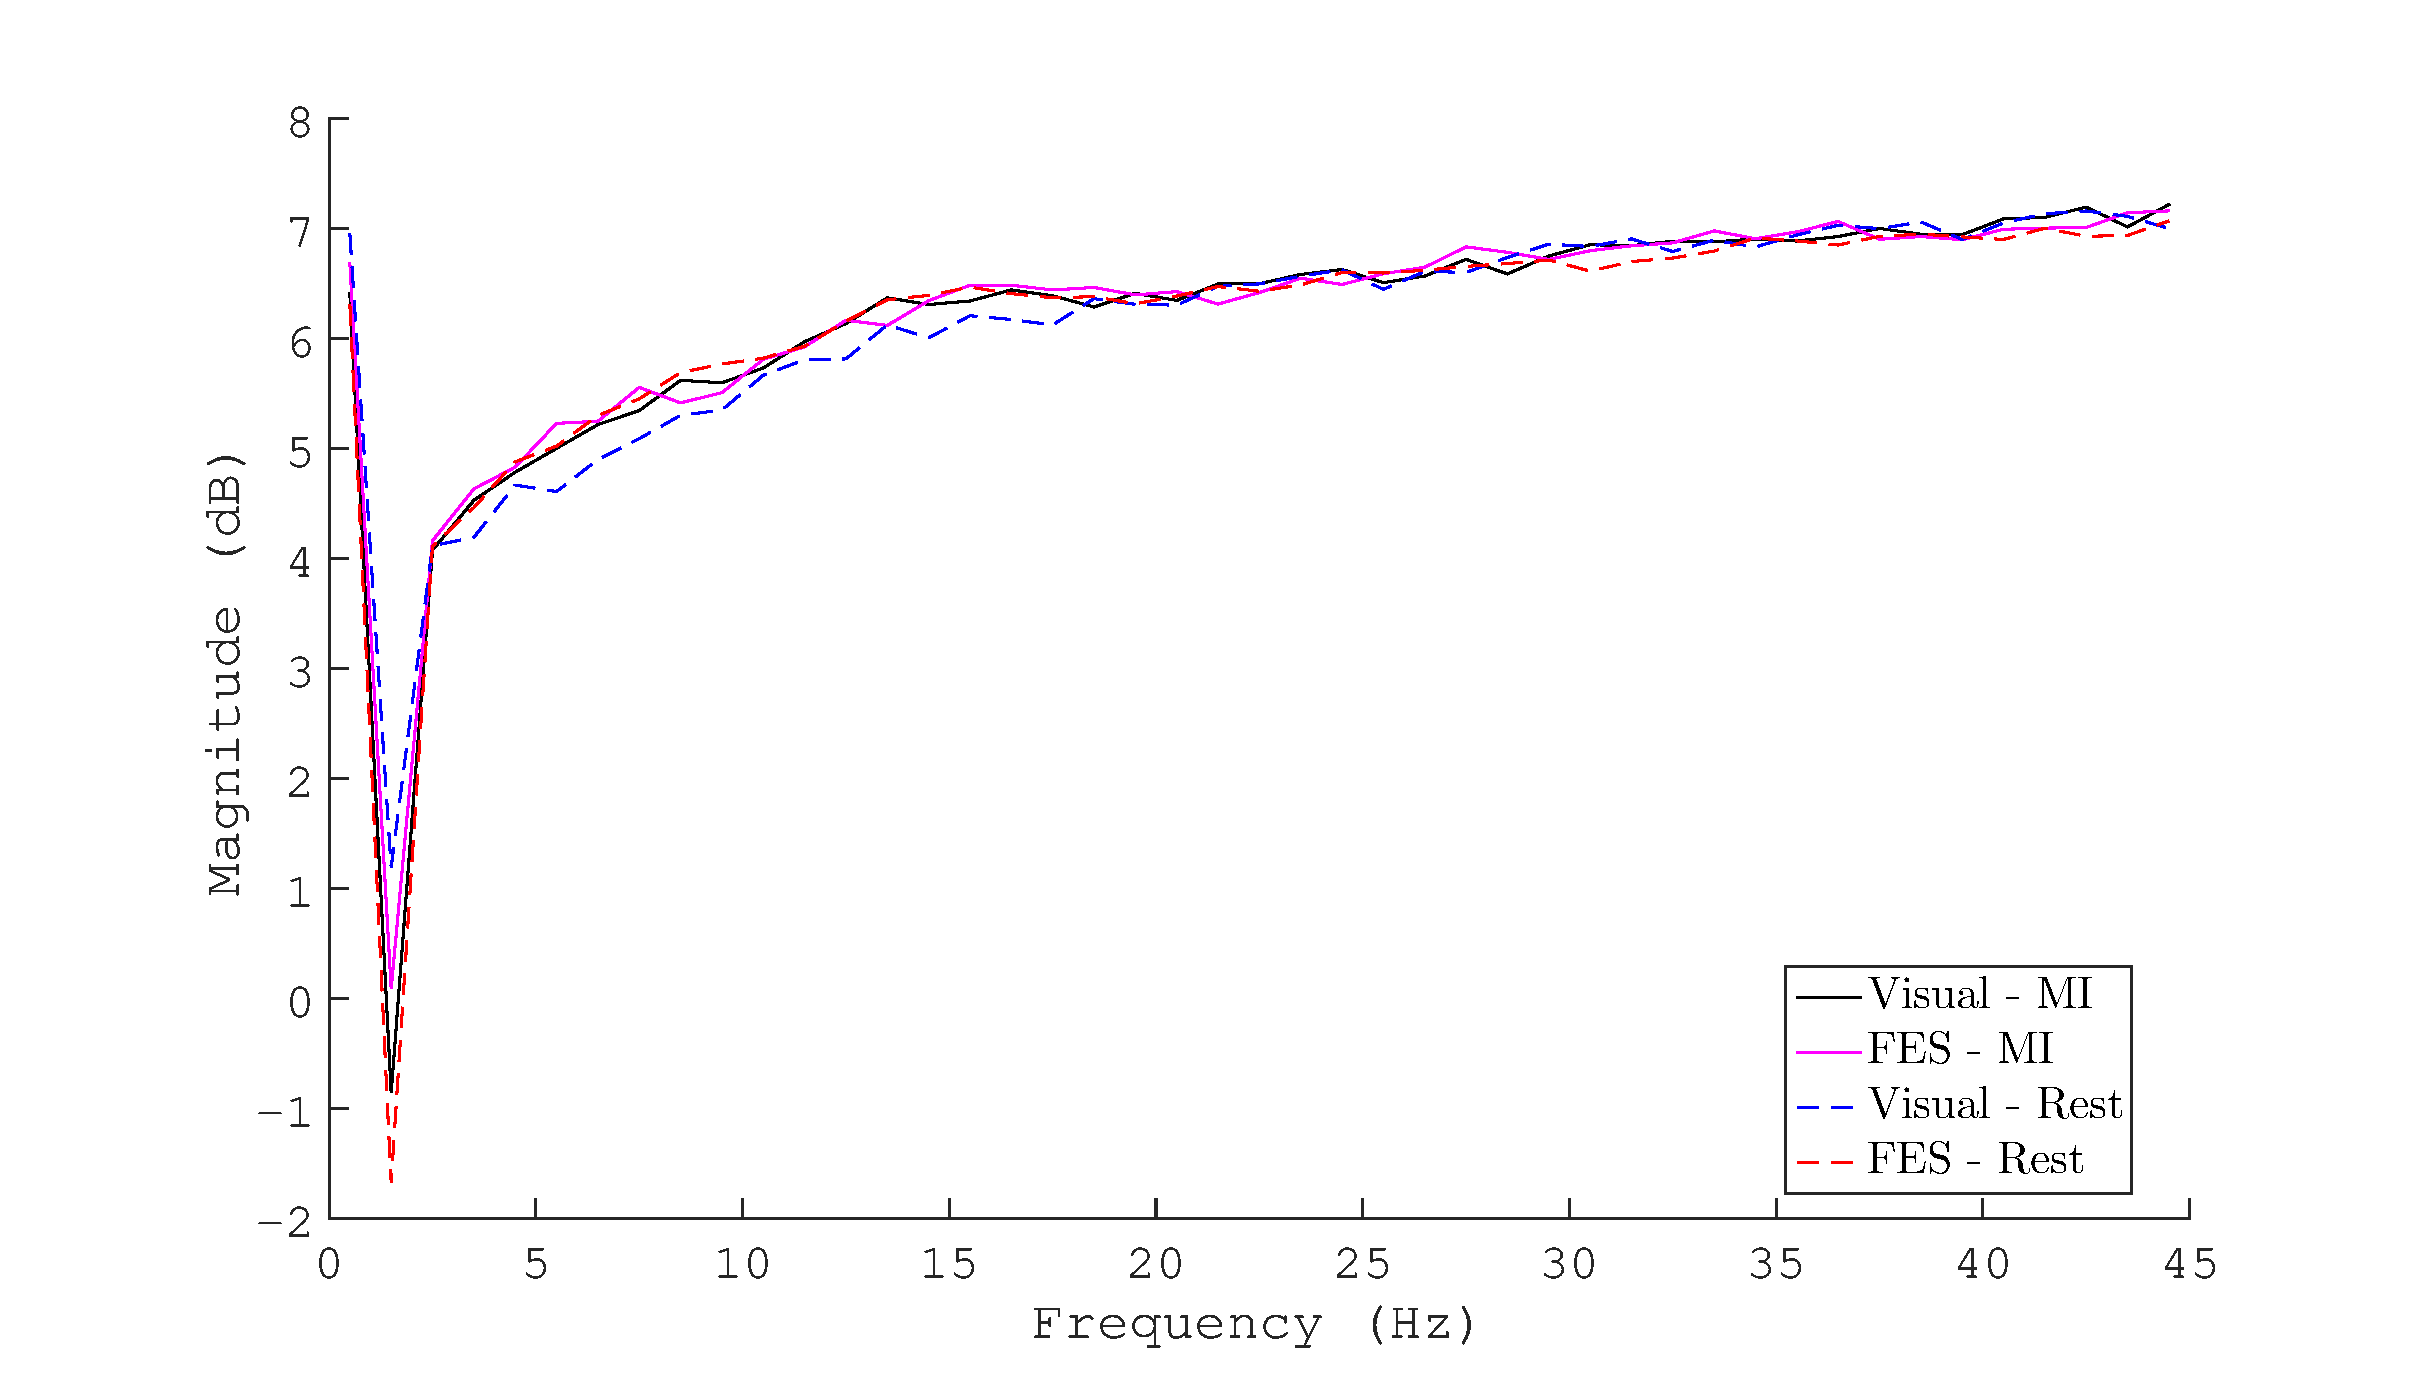
\includegraphics[width=.9\textwidth]{fig/ele12_2.eps}}
\end{center}
\caption{Mean values of the PSD from a given electrode during FES and Visual feedback. Black solid line: Visual + MI. Magenta solid line: FES + MI. Blue dashed line: Visual + Rest. Red dashed line: FES + Rest. Data for session 1 (S1) and session 2 (S2). Note the noise contaminating many of the FES electrodes at ~30Hz.}
\label{meanPSD}
\end{figure*}

\begin{figure*}
   \begin{center}
   \subfloat[Feature selection S1]{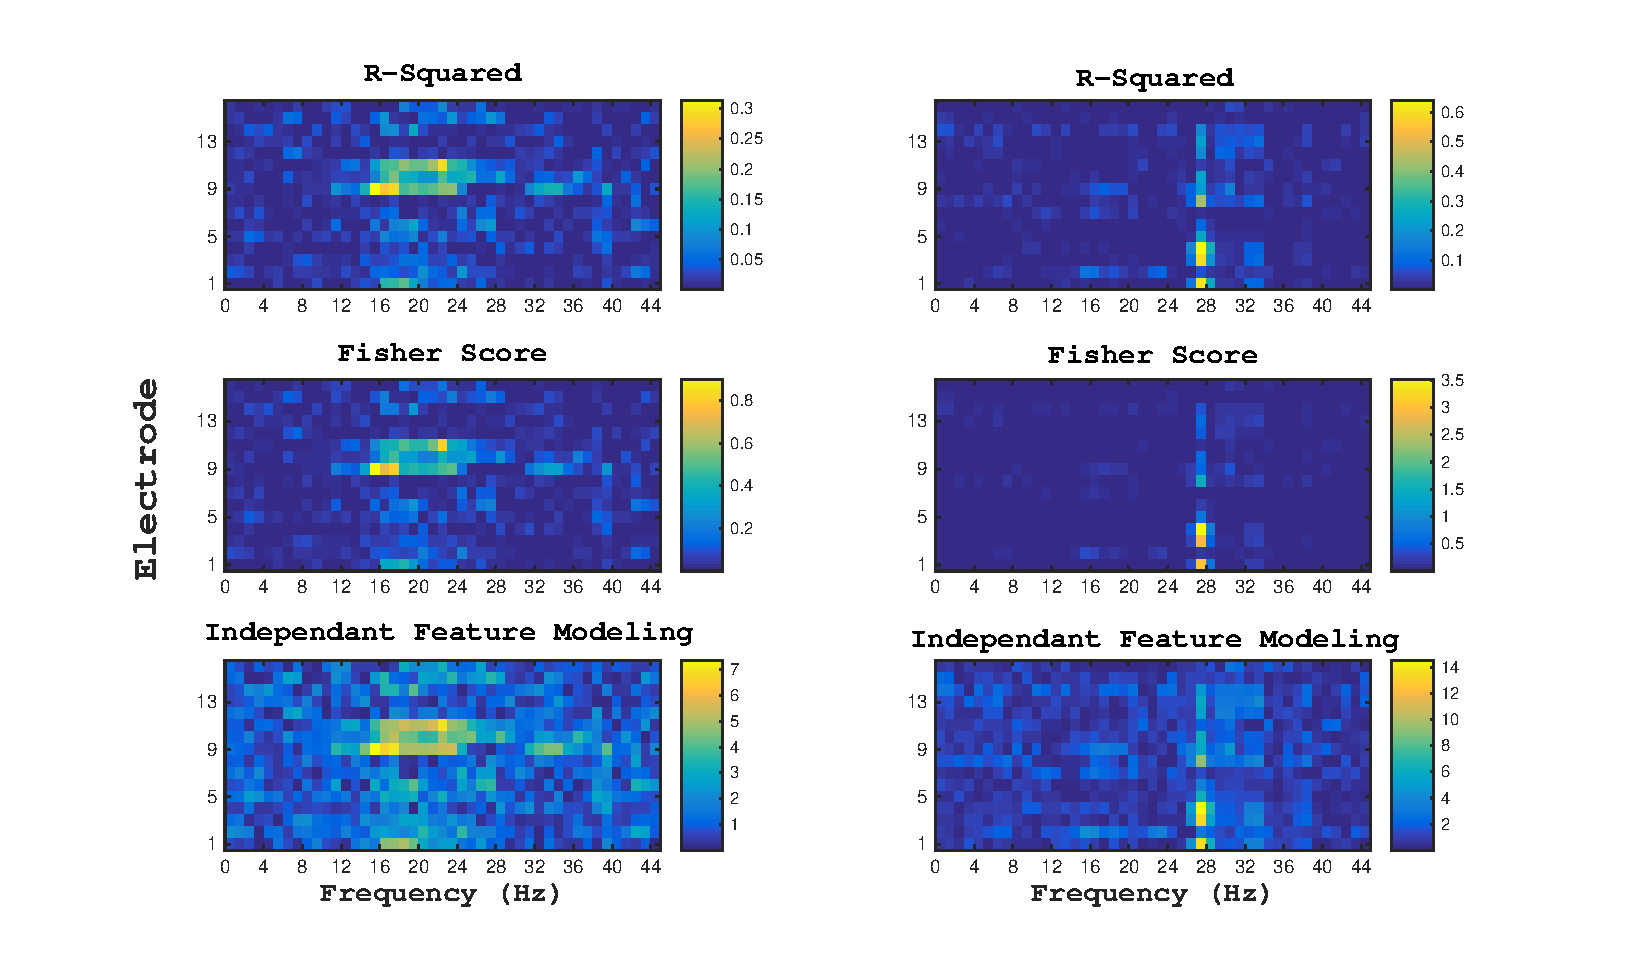
\includegraphics[width=.96\textwidth]{fig/FeatSel.eps}}
   \qquad
    \subfloat[Feature selection S2]{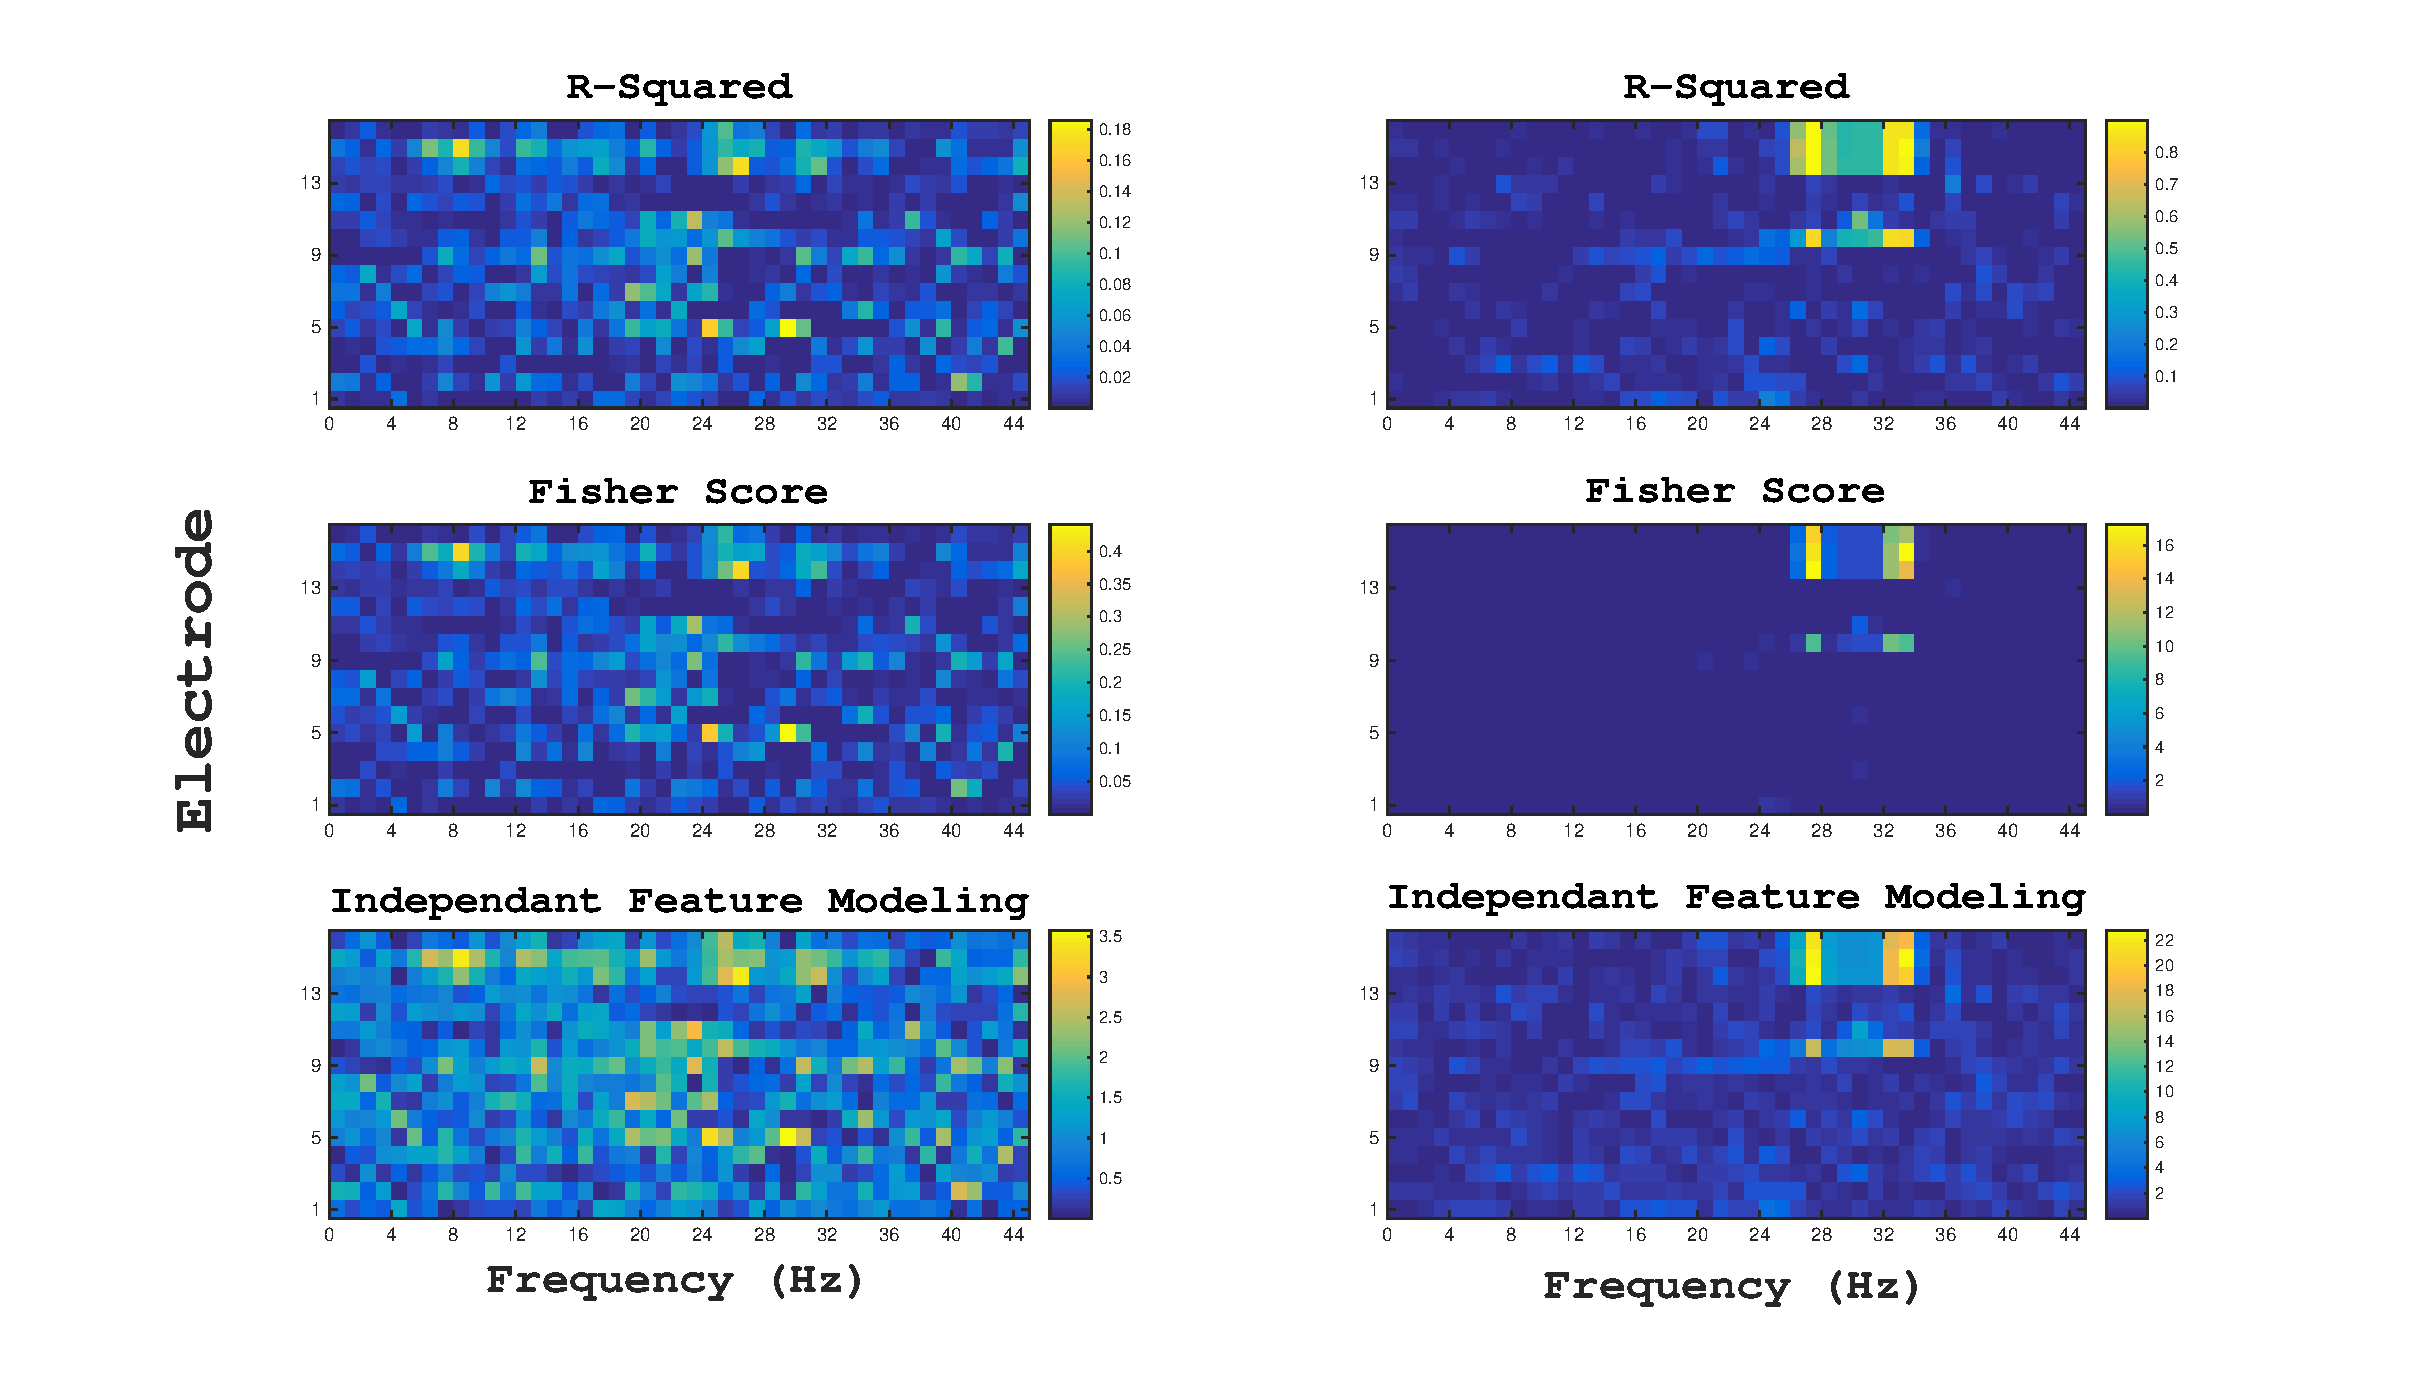
\includegraphics[width=.96\textwidth]{fig/FeatSel_2.eps}}   
   \end{center}
   \caption{Feature selection utilising Pearson product-moment (top row), Fisher score (middle row), and Independent feature modeling (bottom row). Session 1 (a), session 2 (b).}
   \label{featsel1}
\end{figure*}


Features are selected from the unfiltered data in order to accentuate the affect of the high frequency noise on our selection methods (fig.\ref{featsel1}). In order to select meaningful results the extracted features were filtered so as to remove the high frequency noise from the FES channels. After which features are extracted by ranking and selecting features with the largest Fisher score. From each set of 45 possible features we select 4-5 features to be used in our classifier (fig.\ref{topo1}).

 \begin{figure*}
   \centering
   \subfloat[Topological Features S1]{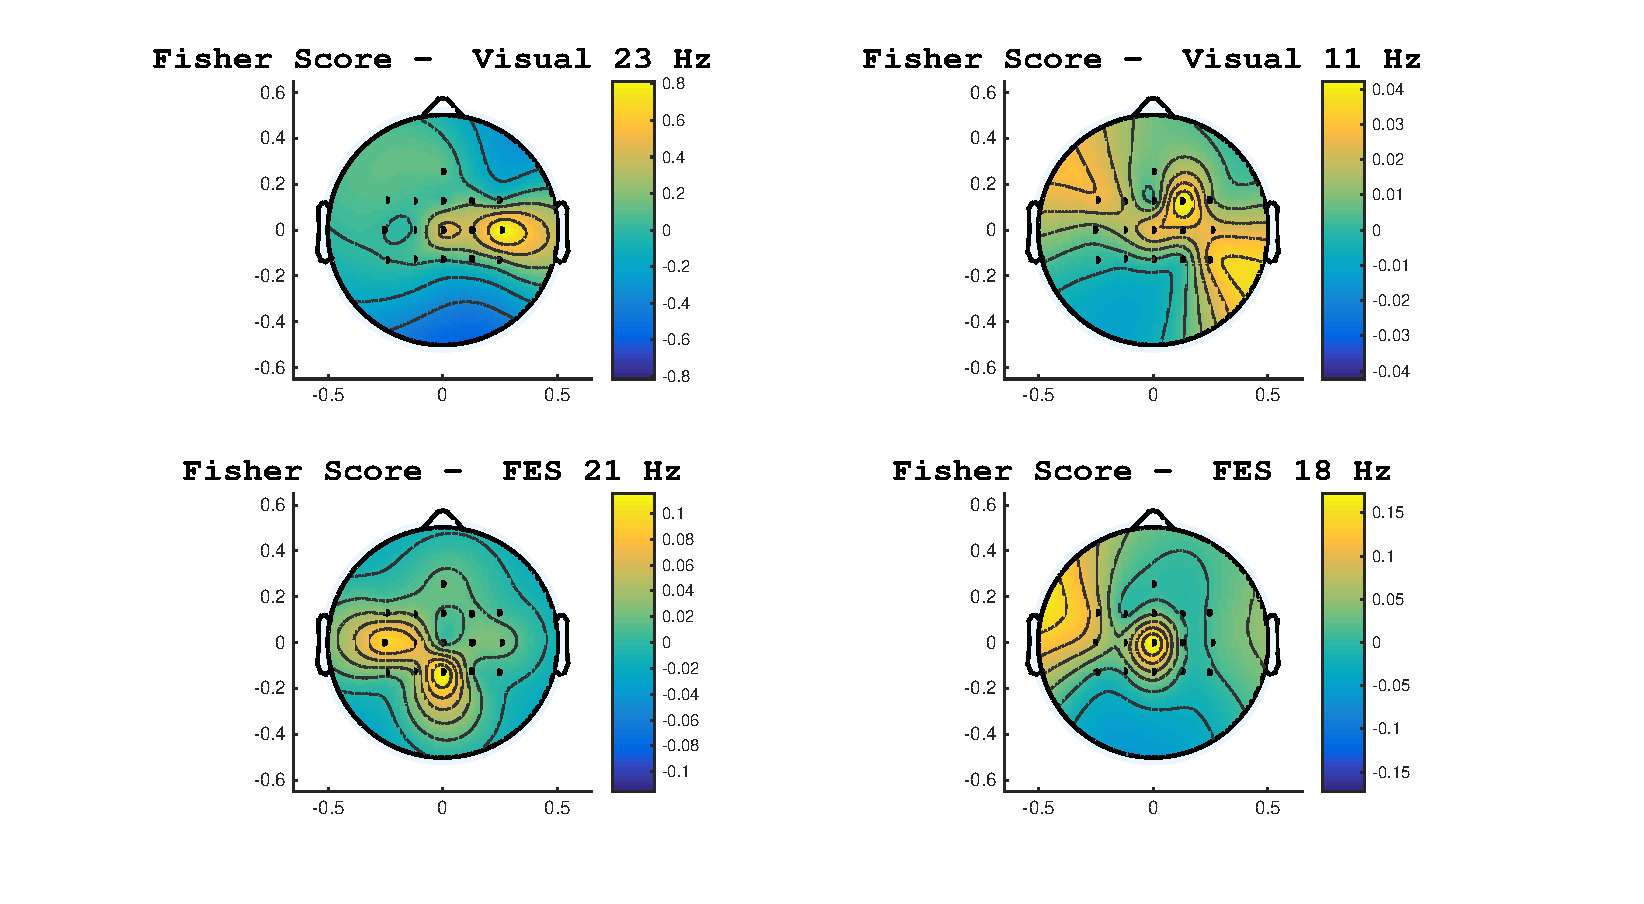
\includegraphics[width=0.95\textwidth, height=0.40\textheight]{fig/fishertopo.eps}}
   \qquad
    \subfloat[Topological Features S2]{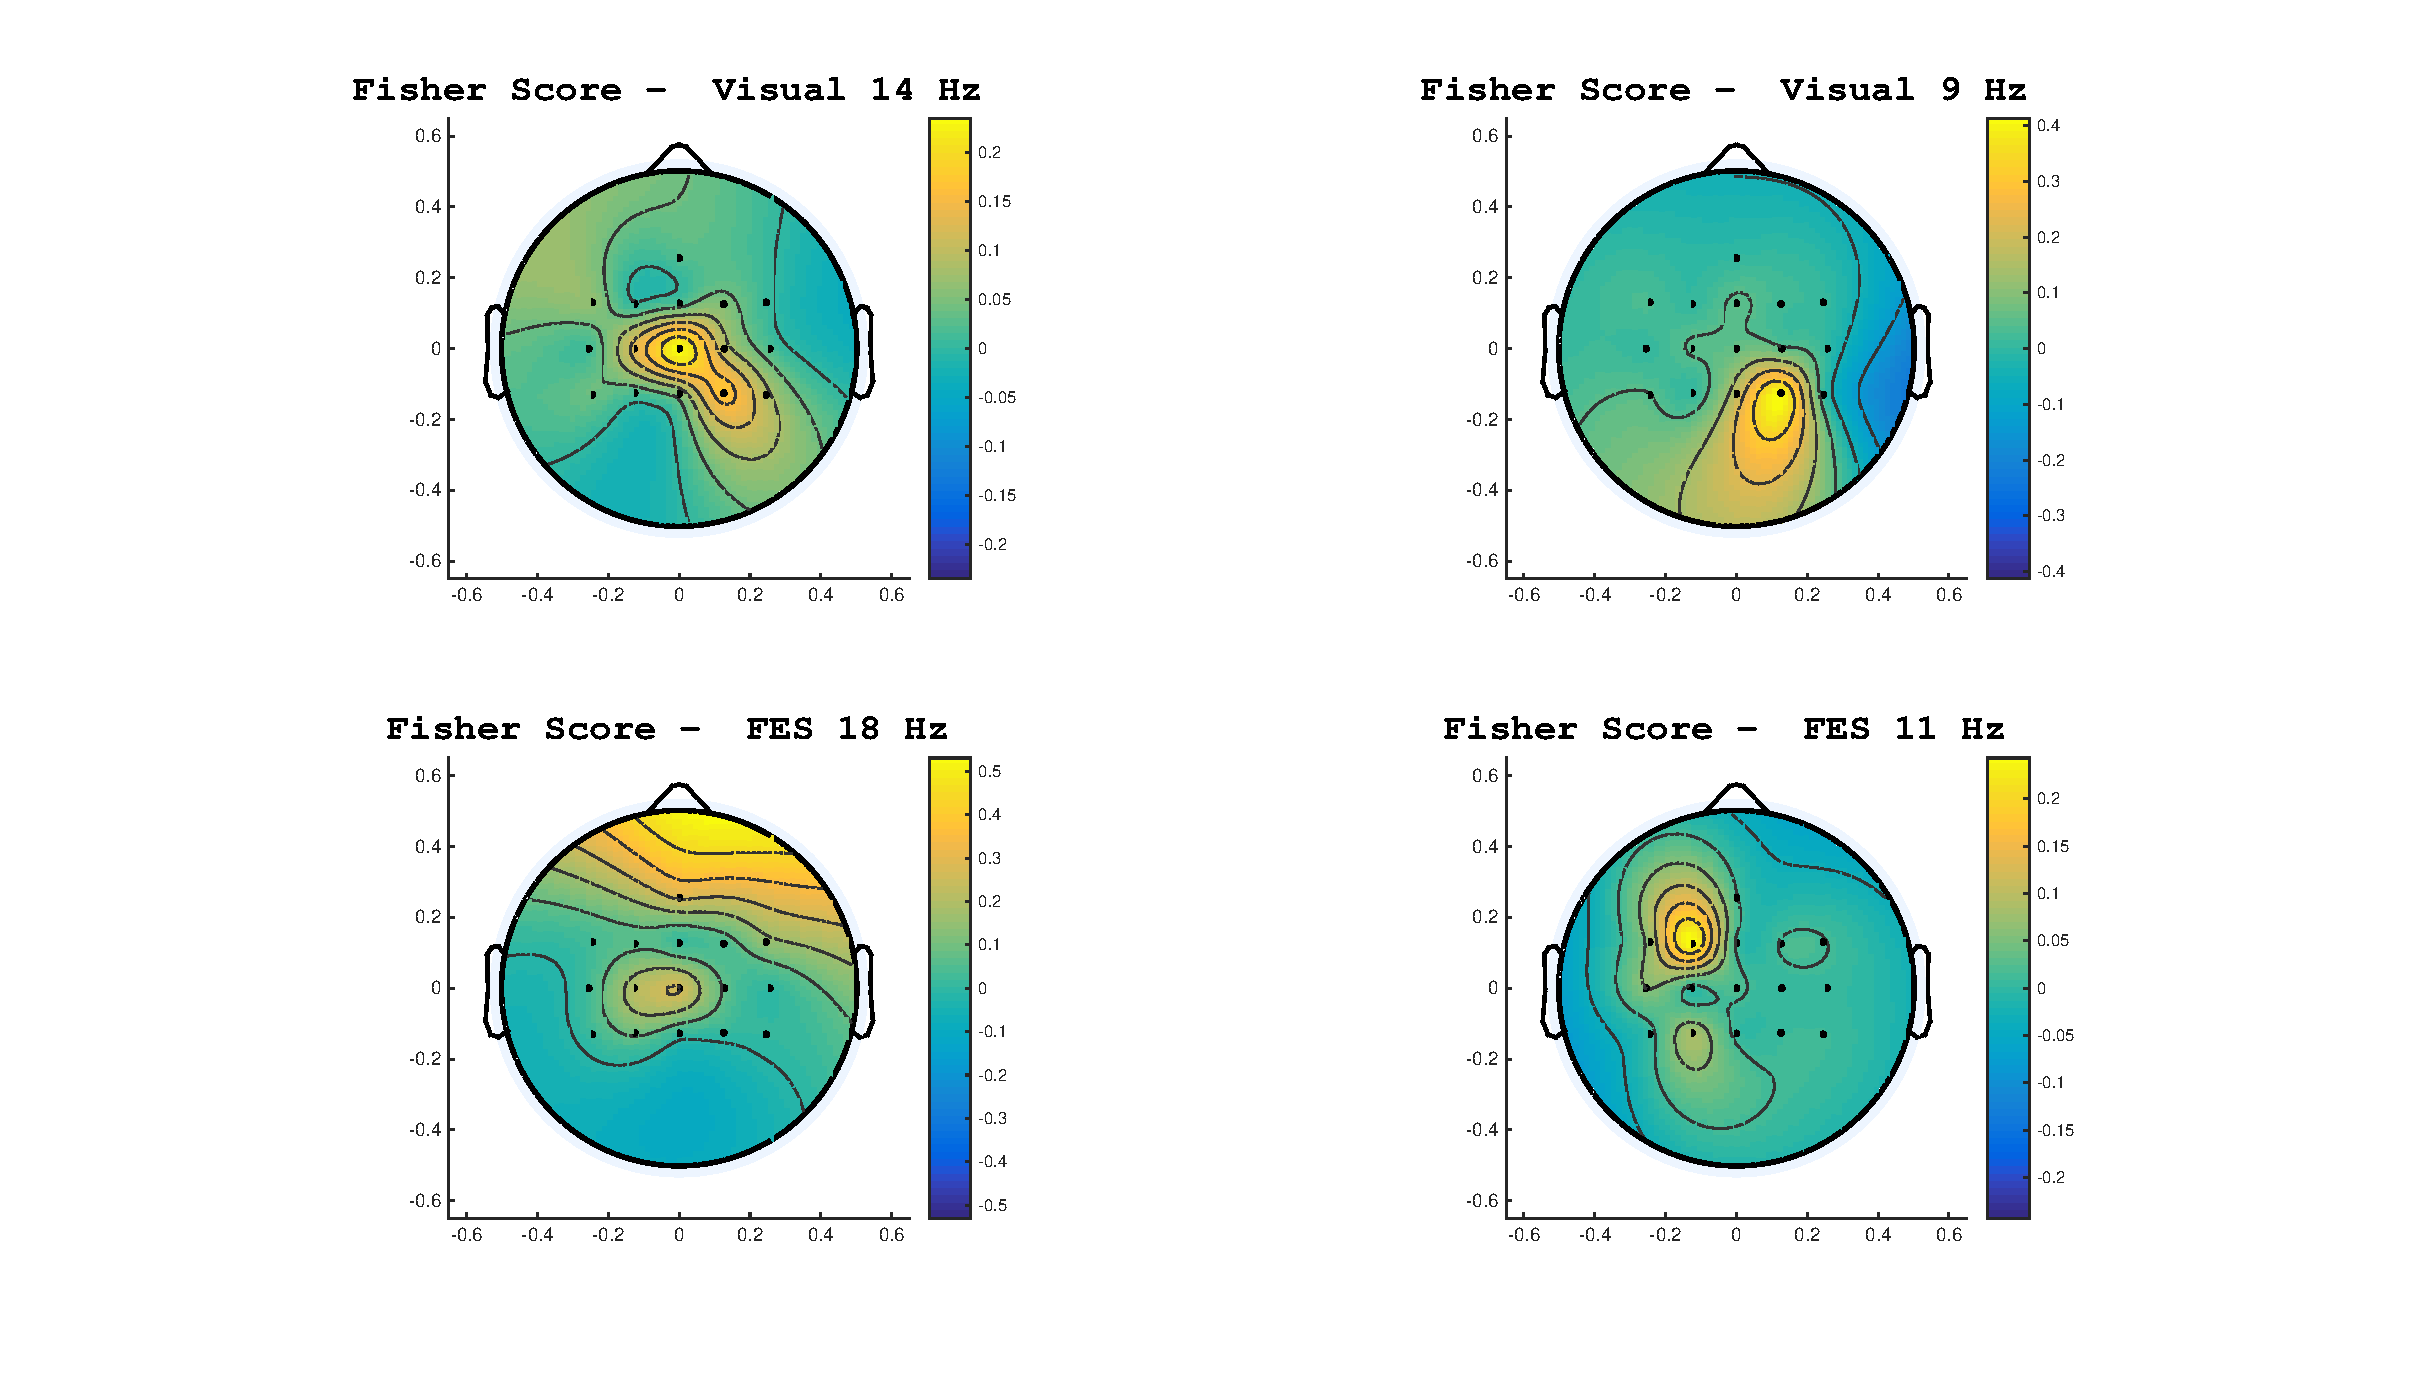
\includegraphics[width=0.96\textwidth, height=0.40\textheight]{fig/fishertopo_2.eps}}
   \caption{Exemplar features selected after processing utilising ranked Fisher scoring. The plot depicts a human skull from above, nose front ears to the side. The regions of high-intensity indicate a strong discriminant power for the given frequency and channel. Data for session 1 (a) and session 2 (b). Note for visual the predominance of higher values towards the right hemisphere indicating a left handed MI during S1.}
   \label{topo1}
\end{figure*}

Classifiers are evaluated utilising a standard cross validation methodology. A subset of the data is arbitrarily declared a training set and the remainder as a test set, this process is repeated twelve times, i.e., from the 120 trials, 10 are selected as the training set and the remainder the test set, this process is repeated until all sets of 10 have been evaluated (fig.\ref{class})

 \begin{figure*}
   \centering
   \subfloat[Classifier Ranking S1]{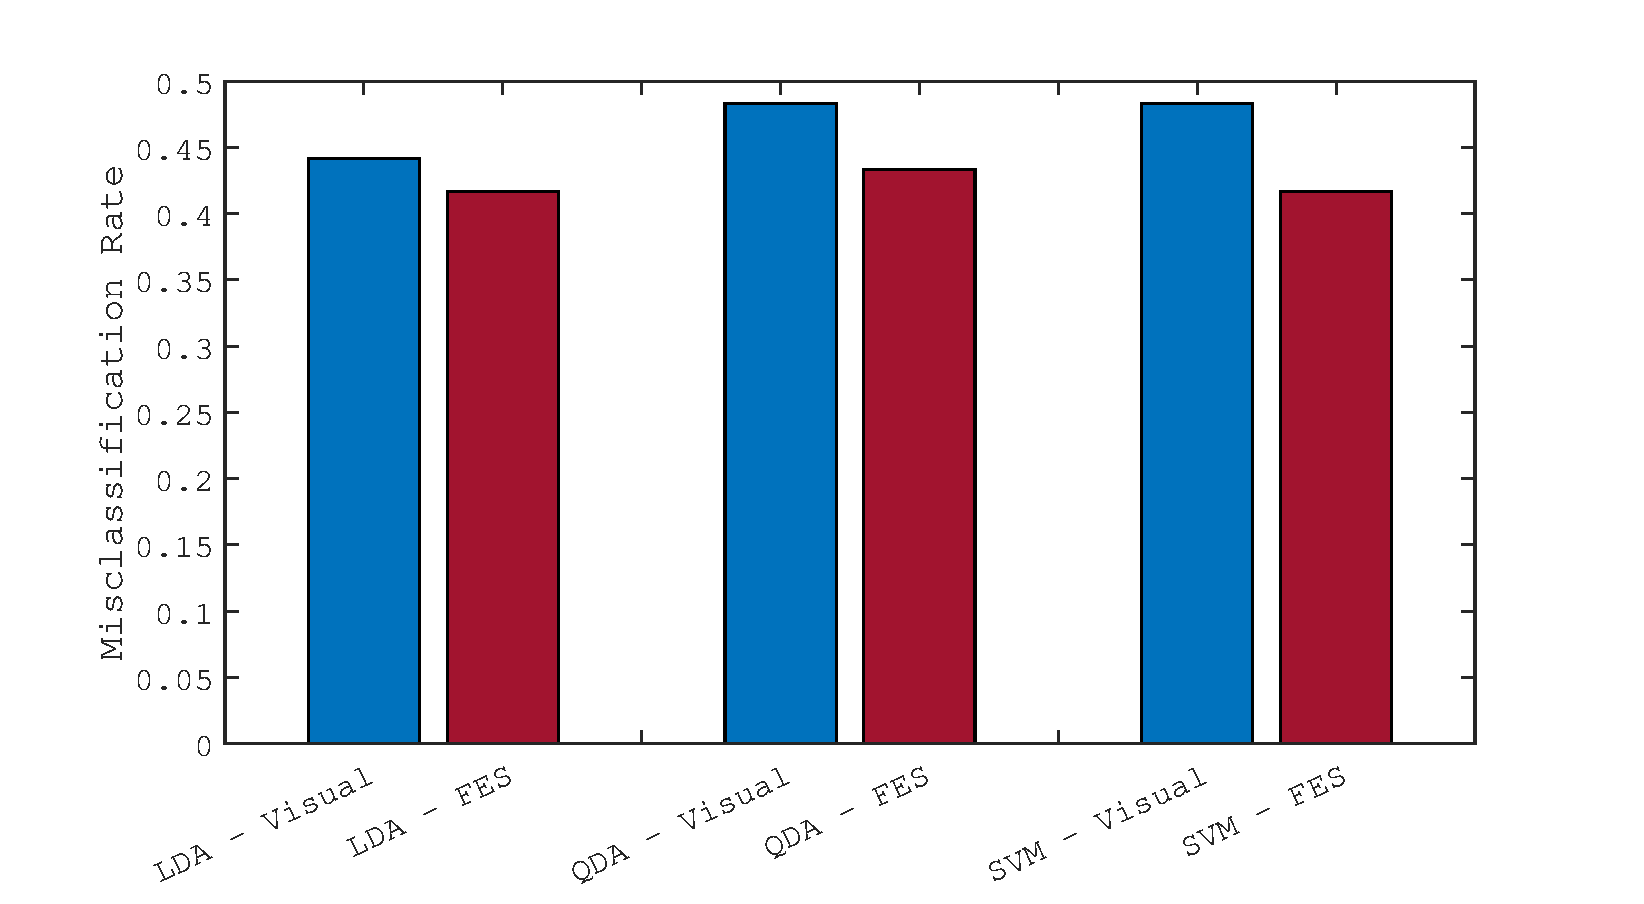
\includegraphics[width=0.95\textwidth, height=0.40\textheight]{fig/classifier.eps}}
   \qquad
    \subfloat[Classifier Ranking S2]{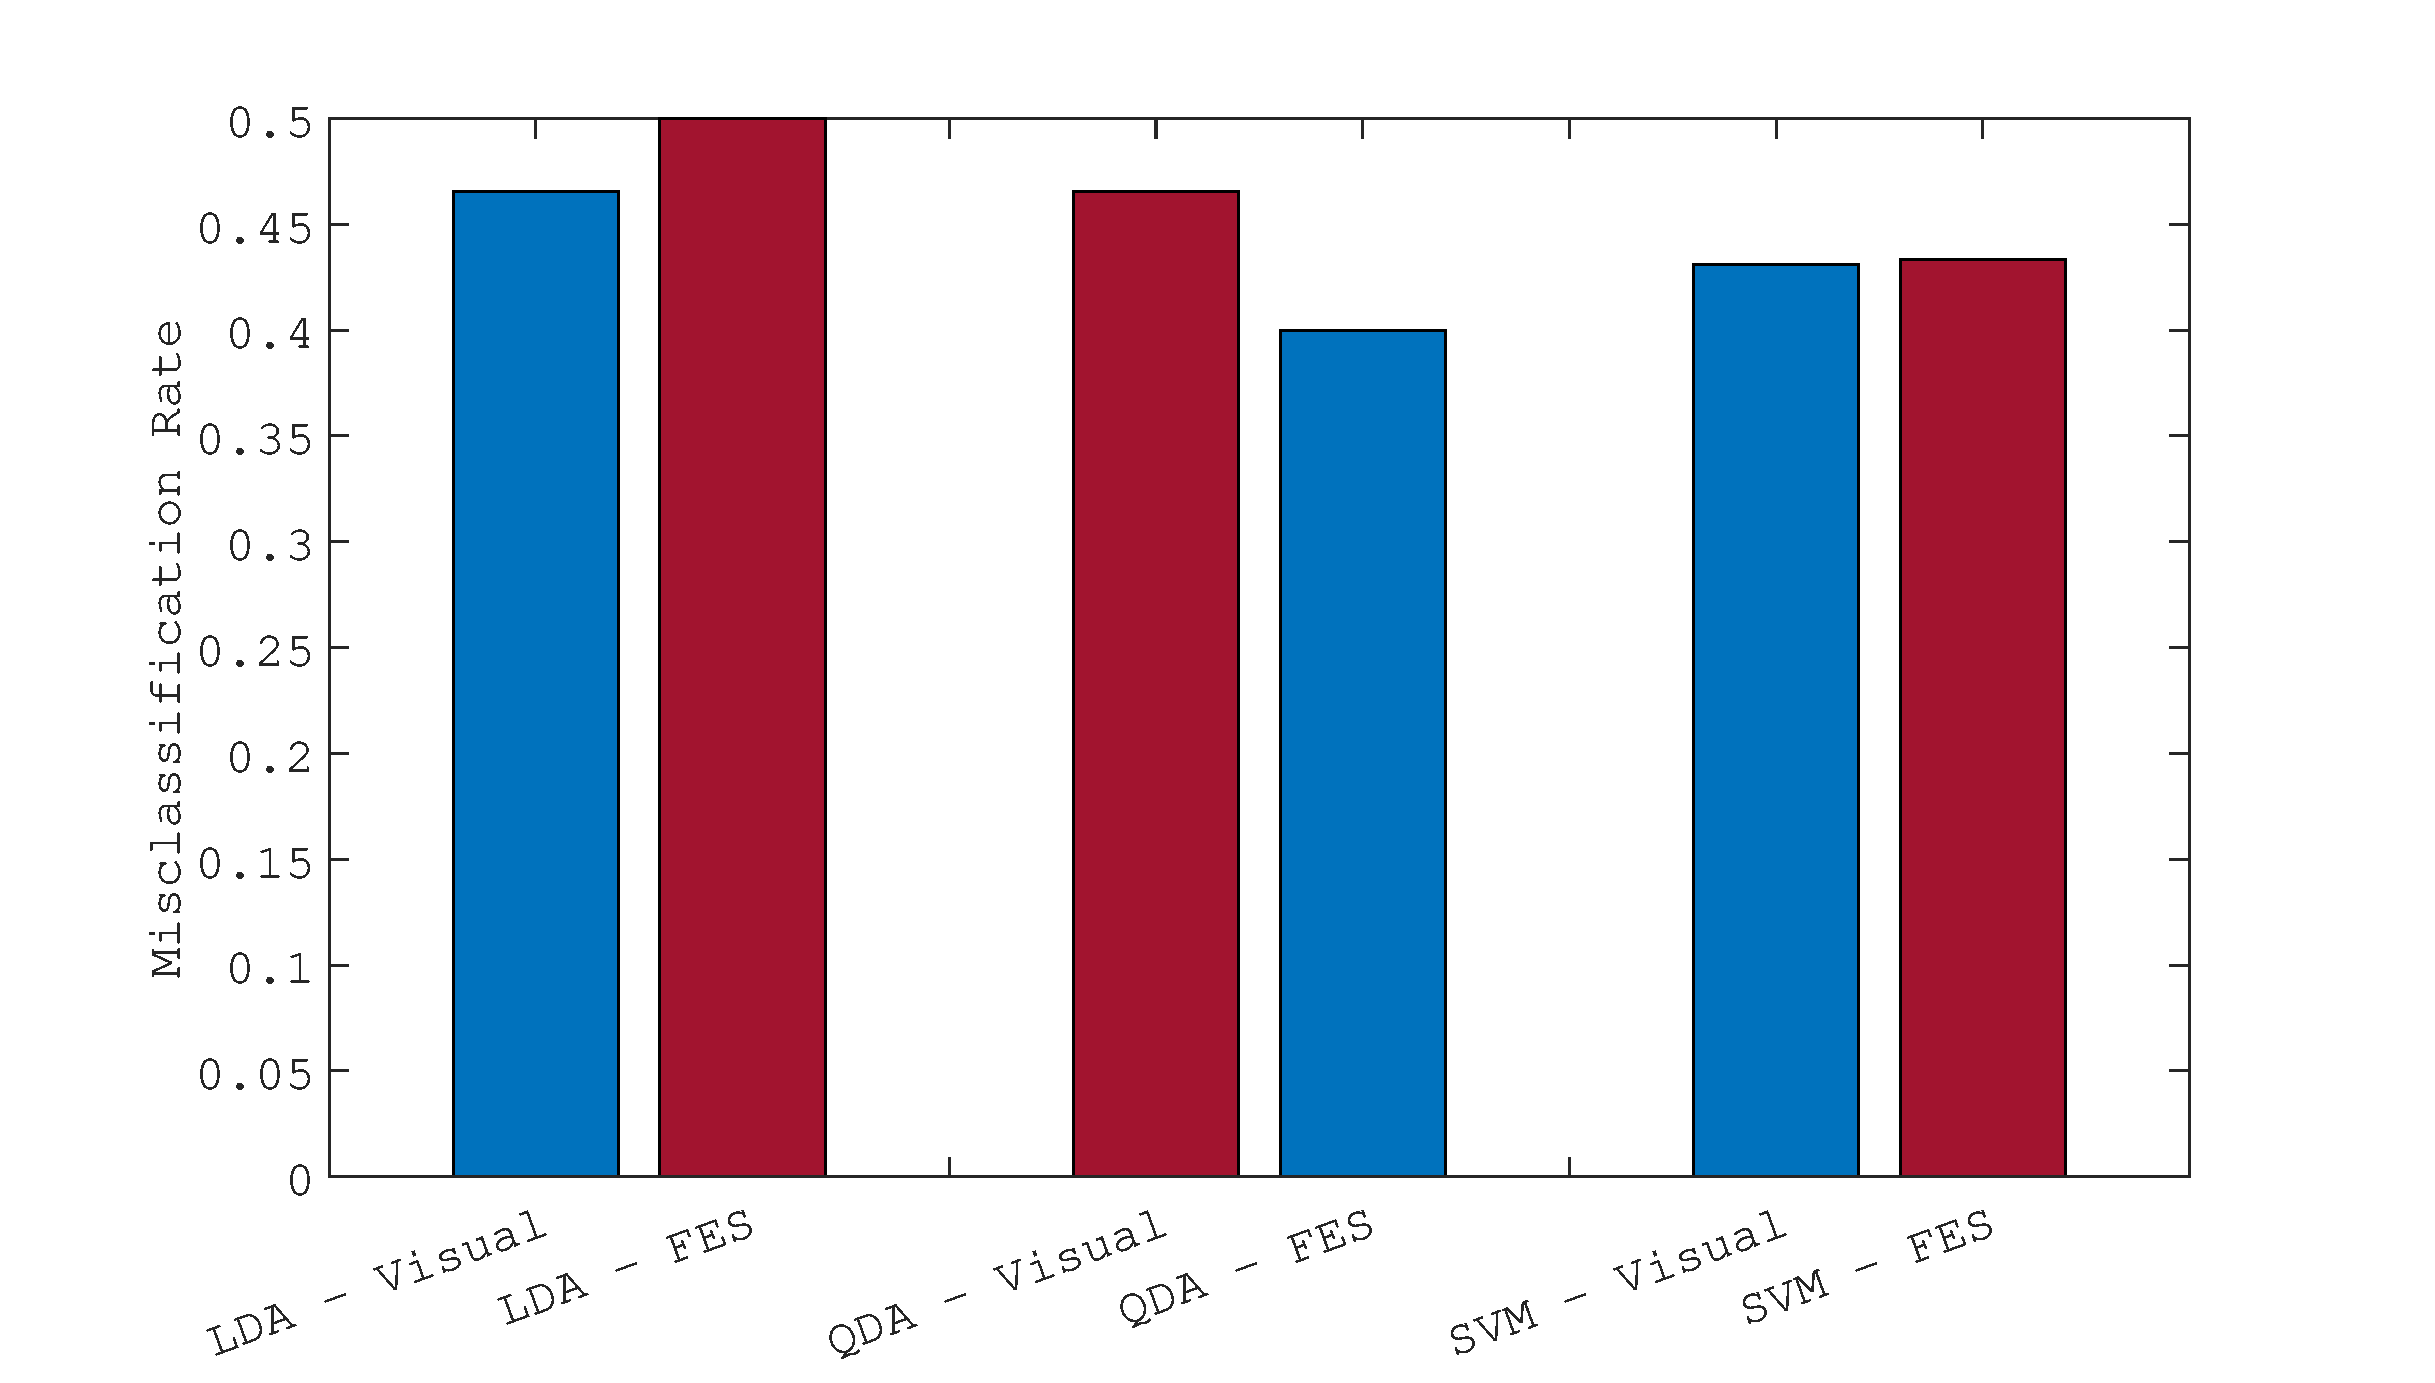
\includegraphics[width=0.95\textwidth, height=0.40\textheight]{fig/classifier_2.eps}}
   \caption{LDA, QDA, and SVM classifiers are examined side by side utilising the same features for both Visual and FES. Session 1 (a), session 2 (b). The y-axis represents the misclassification rate}
   \label{class}
\end{figure*}


We establish a control paradigm by investigating the affect of FES without any MI. Given that this data has no mental task we expect there to be no discriminant power, we establish this by analysis the data as above. We compare the means of the FES - No MI PSD with its counterpart (fig.\ref{meanPSD2}). Performing feature selection via our outlined statistical tests (fig.\ref{featsel2}).

\begin{figure*}
\begin{center}
\subfloat[Ch 10 PSD S3]{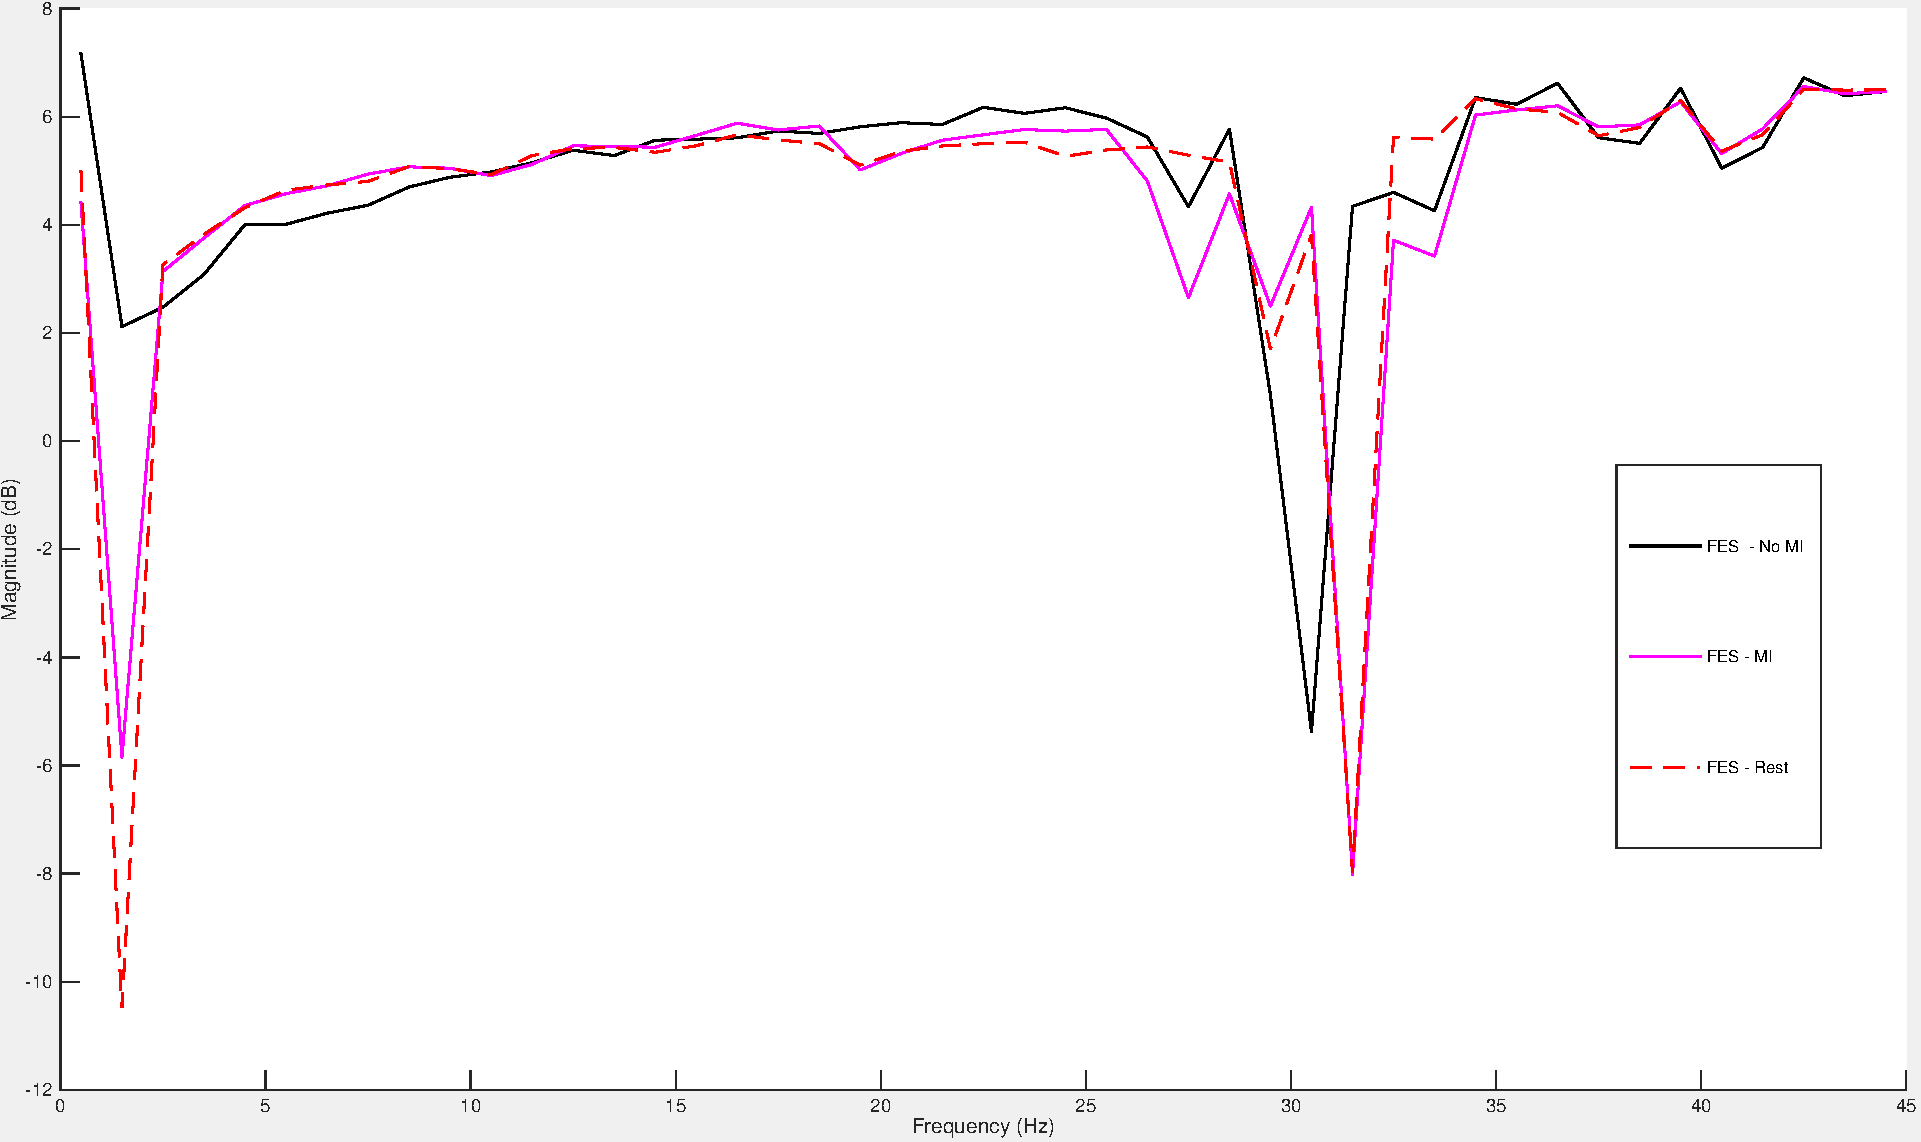
\includegraphics[width=.30\textwidth, height=40mm]{fig/ele10_3.pdf}}
\qquad
\subfloat[Ch 11 PSD S3]{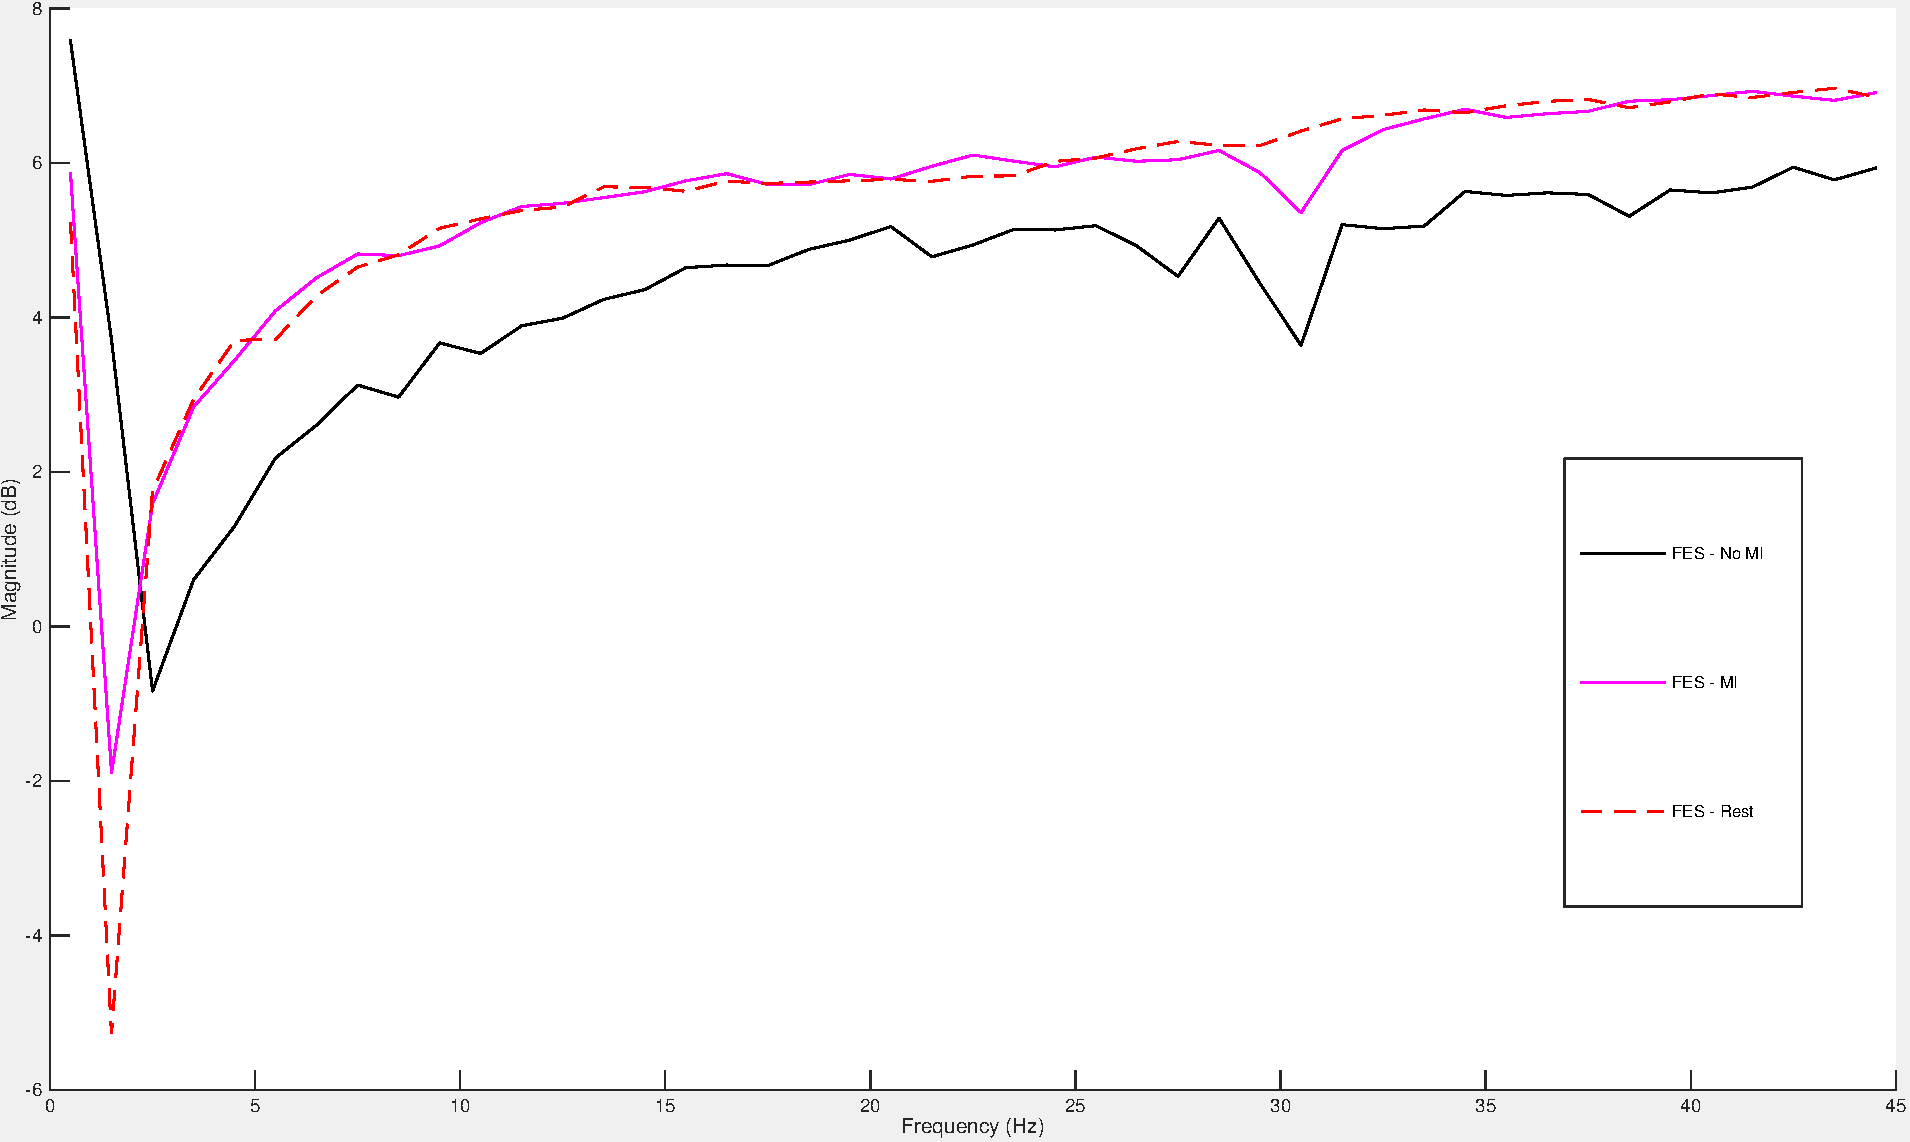
\includegraphics[width=.30\textwidth, height=40mm]{fig/ele11_3.pdf}}
\qquad
\subfloat[Ch 12 PSD S3]{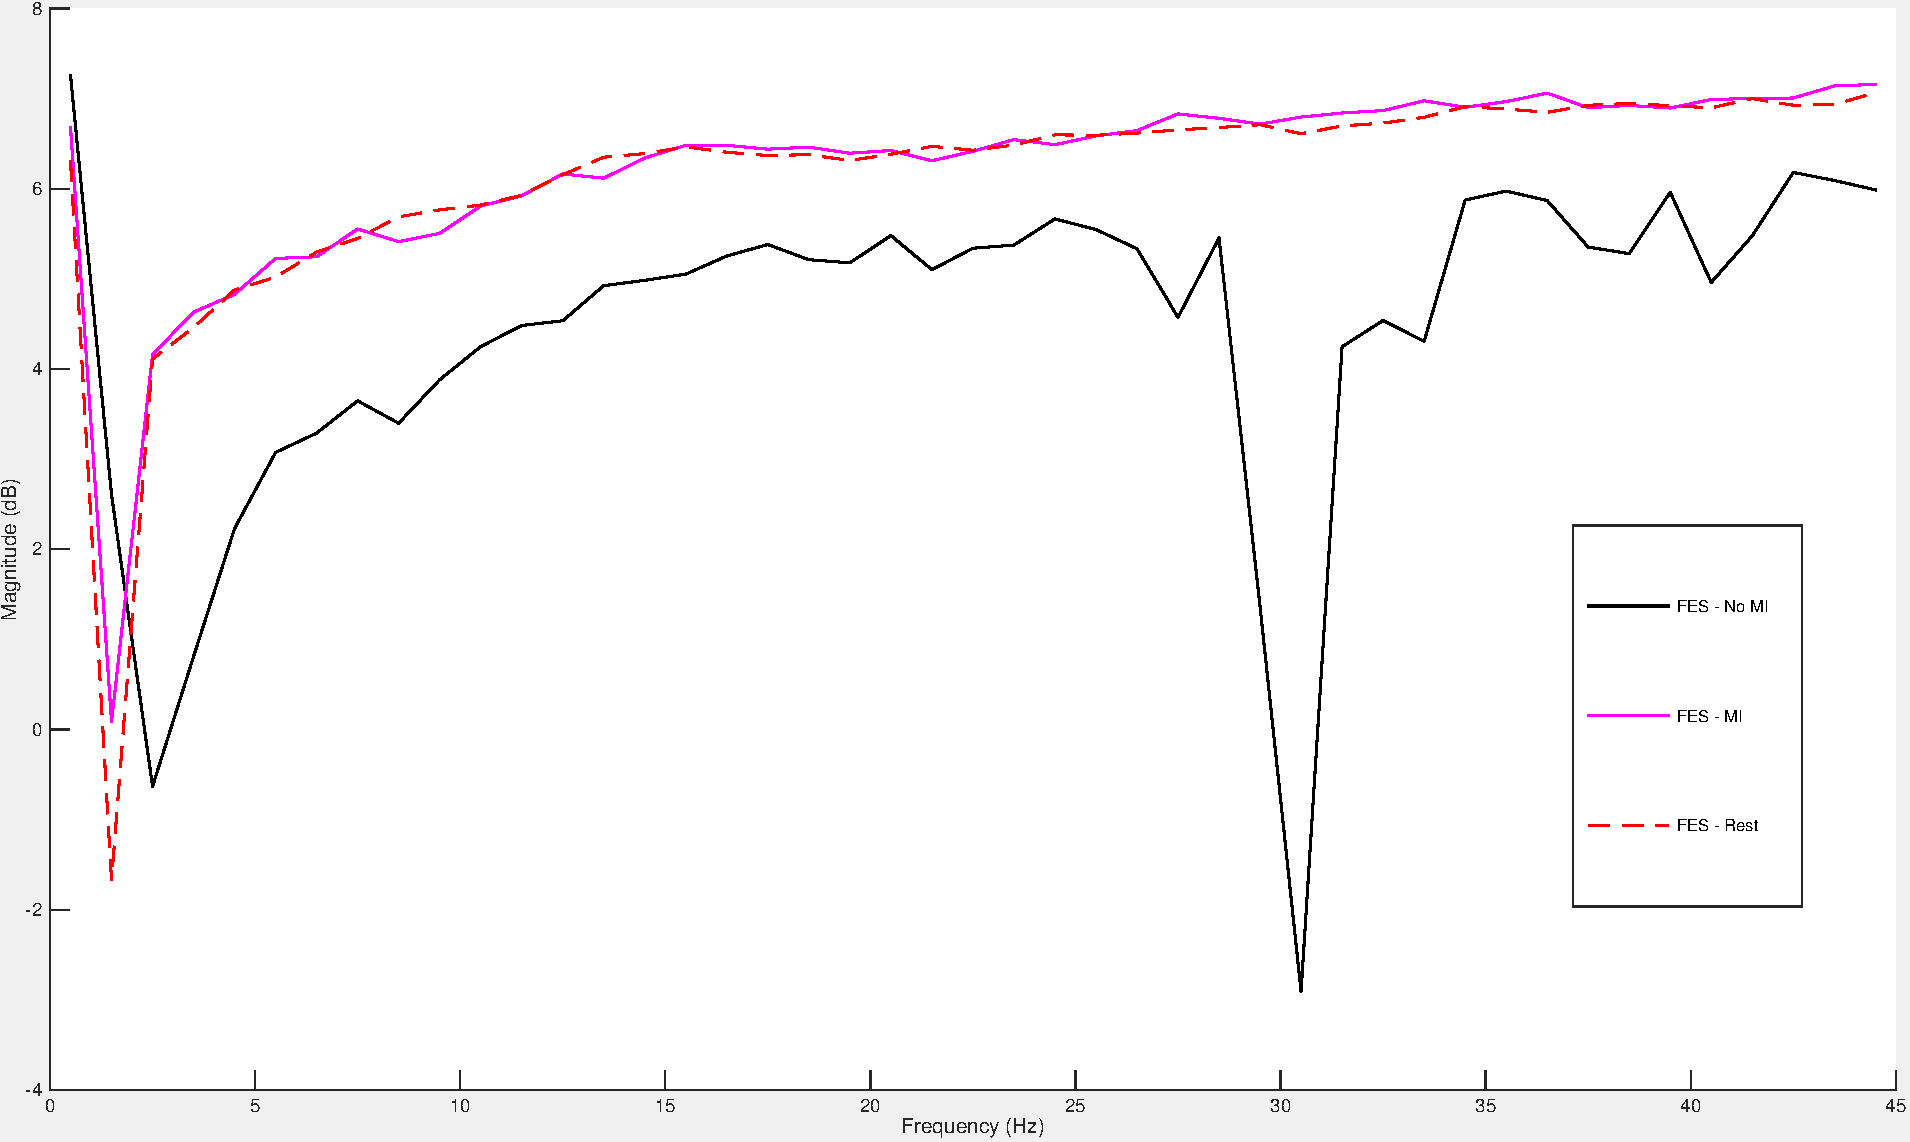
\includegraphics[width=.30\textwidth, height=40mm]{fig/ele12_3.pdf}}
\qquad
\end{center}
\caption{Mean values of the PSD from the FES - No MI (Black solid line), and the FES - MI, and Rest (Magenta solid line, red dashed line - respectively). Data is from the third session (S3).}
\label{meanPSD2}
\end{figure*}

 \begin{figure*}
   \centering
   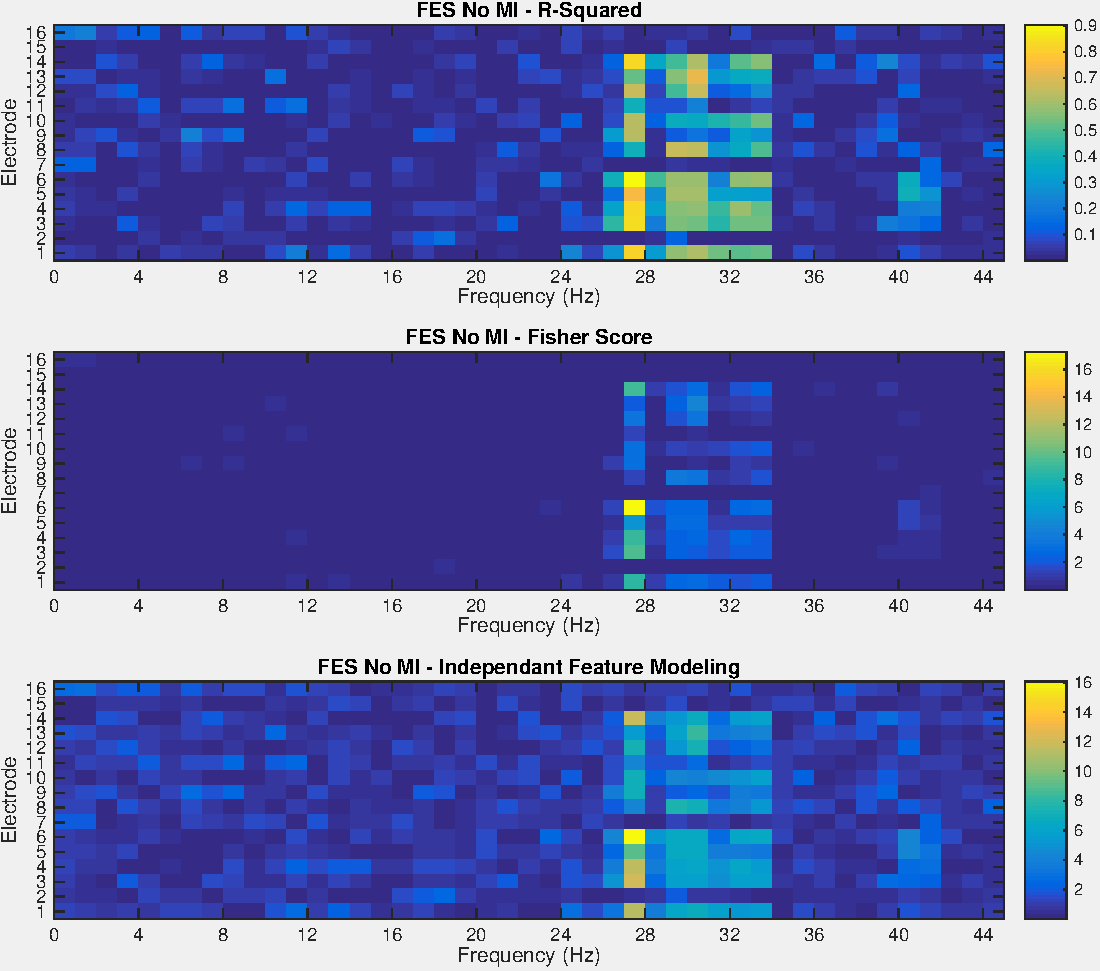
\includegraphics[width=.77\textwidth, height=80mm]{fig/FeatSel_3.pdf}
   \caption{Feature selection utilising Pearson product-moment (top row), Fisher score (middle row), and Independent feature modeling (bottom row). Session 3. Note the lack of any discriminant features beyond noise present at 30 Hz.}
    \label{featsel2}
\end{figure*}

\subsection{Subject 2}

\section{Discussion}

Examining the exemplar power spectral densities (fig.\ref{meanPSD}) several factors are immediately obvious. Foremost, EEG signals are very sensitive to any external noise sources. High frequency noise can contaminate the recording electrodes from a multitude of sources, FES, eye-blinks, jaw clenching, and external radiation, while this is is hardly a comprehensive list of all contaminants it presents some of the significant sources which must dealt with to extract meaningful data from EEG measurements. Next it is evident that the variance between any given rest or MI task is quite minimal, this can be ascertained from both a visual inspection of (fig.\ref{meanPSD}) or statistically from (fig.\ref{featsel1}).

In attempting to quantify the features of interest caution must be taken so as to not assume that a feature of interest in one session will remain stable through time. Closer inspection of (fig.\ref{featsel1}) demonstrates this phenomenon, features which during the first session provided a relatively strong response across all statistical tests are no longer of any use during the next experimental session. This phenomena aptly nicknamed \lq feature drift\rq, is likely the result of a multitude of physiological alterations to the brain state as a function of time, further these features can be altered depending on the subjects brain state (e.x., fatigue \cite{PSYP:PSYP1329}). 

Motor imagery is associated predominantly with the Mu band (7.5 - 12.5 Hz) \cite{Pfurtscheller:2006aa} of brain wave activity, although the variance in the activity is fairly large and some experiments find subjects who respond to MI task primarily in the beta (16 - 31 Hz) frequency band \cite{Pfurtscheller:1997aa}. We may thus conclude that activity in the region of either the Mu or Beta frequency bands can potentially be attributed to the MI task \cite{Formaggio:2010aa}. 

Movement of either the left or right hand maps to brain regions contralateral to the hand (i.e., left hand - right hemisphere) \cite{Pfurtscheller:1997aa}. Thus we should expect to find a predominance of event-related desynchronization (ERD) over the right hemisphere for left handed subject and vice versa for right handed subjects \cite{Solodkin01112004}. Topological maps shown in (fig.\ref{topo1}a) are in agreement with this finding for visual data, but FES shows a more central activation, this may indicate that movement it self took place during these trials where the pattern of activation will shift from unilateral to bilateral activation \cite{Pfurtscheller:1997aa}. Session 2 (fig.\ref{topo1}b) lacks the same degree of contralateral activation, at 20 and 14 Hz some contralateral activation is present but lacks the same degree of certainty. Neither of the two FES sessions demonstrated any strong contralateral activation for subject 1. 

The control FES session gave data in-line with our assumptions that FES alone would have little to no affect while the subject was at rest. Note in (fig.\ref{meanPSD2}) that the signal closely follows the FES - Rest paradigm. We reinforce this suspicion by evaluating the data via our statistical analysis methods (fig.\ref{featsel2}, with the exception of the noise present at higher frequencies it is immediately obvious that there are no discriminant features utilising FES alone. 

Classifiers demonstrated fairly equivalent accuracy rates. FES on average performed worse than visual for subject 1, which should be expected from the quality of features that could be extracted from each data set. LDA performed similar to QDA which implies the covariance matrix between the data are numerically similar. Of particular interest with regard to our classifiers is the SVM classifier. As stated a linear kernel was adopted during our analysis, a common practice which will often yield better classification results for EEG data is to exchange the SMO method which is bound by a linear kernel for the radial basis function (eq.\ref{radial} \cite{xu2011robot}). 
\begin{equation}
k(x_i,x_j) = \exp(\frac{-\norm{x_i - x_j}^2}{2\sigma^2})
\label{radial}
\end{equation}

This non-linear kernel allows SVM more flexibility when choosing the hyperplane through higher dimension space thereby increasing the robustness of the classification method. Is is thus of note that despite our intentional use of a weaker kernel SVM still outperformed all other classifiers during sessions where features extracted were most likely of high quality (fig.\ref{class}a). 

\section{Conclusion}


%\begin{*figure}
%\begin{center}
%\subfloat[]{\includegraphics[scale=0.45]{__.eps}\label{__}}
%\quad
%\subfloat[]{\includegraphics[scale=0.45]{__.eps}\label{__}}
%\end{center}
%\caption{__}
%\label{__}
%\end{figure*}
%
%\begin{*figure}
%\begin{center}
%\includegraphics[scale=0.6]{__.eps}
%\caption{__}
%\label{__}
%\end{center}
%\end{figure*}



\end{multicols}

\newpage
\bibliographystyle{plain}
\bibliography{citations/bmi}

\end{document}